%
% LaTeX template for prepartion of submissions to PLDI'15
%
% Requires sigplanconf style file provided on PLDI'15 web site
%
\documentclass[pldi,nocopyrightspace]{sigplanconf}

%
% the following standard packages may be helpful, but are not required
%
%\usepackage{SIunits}            % typset units correctly
\usepackage{courier}            % standard fixed width font
\usepackage[scaled]{helvet} % see www.ctan.org/get/macros/latex/required/psnfss/psnfss2e.pdf
\usepackage{url}                  % format URLs
\usepackage{listings}          % format code
\usepackage{enumitem}      % adjust spacing in enums
\usepackage[colorlinks=true,allcolors=blue,breaklinks,draft=false]{hyperref}   % hyperlinks, including DOIs and URLs in bibliography
\usepackage[tight]{subfigure}
\usepackage{xspace}
\usepackage{graphicx}
\usepackage{mathtools}
\usepackage{mathpartir}
\usepackage{amssymb}
\usepackage{amsmath}
\usepackage{textcomp}

\usepackage[usenames,dvipsnames,svgnames,table]{xcolor}
\usepackage{amsthm}
\usepackage[ruled,vlined,linesnumbered]{algorithm2e}
%==============================================================================


\newcommand{\cf}[1]{{\small\tt #1}}
\newcommand{\rcf}[1]{\mathrm{\cf{#1}}}
\newcommand{\conj}{~\wedge~}
\definecolor{darkgreen}{rgb}{0,0.5,0}
\definecolor{darkred}{rgb}{0.5,0,0}
\newcommand{\KC}[1]{{\textcolor{red}{{KC: #1}}}}
\newcommand{\GK}[1]{{\textcolor{red}{{GK: #1}}}}


%%%%%%%%%%%%%%%%%%%%%%%%%%%%%%%%%%%%%%%%%%%%%%%%%%%%
%%% General
\font\nine=cmr9

\font\ninerm=cmr9
\font\ninebf=cmbx9
\font\nineit=cmti9
\font\ninesl=cmsl9
\font\ninett=cmtt9
\font\ninemi=cmmi9  \skewchar\ninemi='177
\font\ninesy=cmsy9  \skewchar\ninesy='60
\font\nineex=cmex10

%%%%%%%%%%%%%%%%%%%%%%%
%% Math Fonts

\font\mathninerm=cmr9
\font\mathninei=cmmi9
\font\mathninesy=cmsy9


\def\ninepoint{\def\rm{\fam0\ninerm}%
\textfont0=\mathninerm\scriptfont0=\mathsevenrm\scriptscriptfont0=\mathfiverm%
\textfont1=\mathninei\scriptfont1=\mathseveni\scriptscriptfont1=\mathfivei%
\textfont2=\mathninesy\scriptfont2=\mathsevensy\scriptscriptfont2=\mathfivesy%
\textfont3=\tenex
\let\sc=\sevenrm
 \def\it{\fam\itfam\nineit}%
  \textfont\itfam=\nineit
  \def\bf{\fam\bffam\ninebf}%
  \textfont\bffam=\ninebf
  \def\tt{\fam\ttfam\ninett}%
  \textfont\ttfam=\ninett
  \setbox\strutbox=\hbox{\vrule height9pt depth4pt width0pt}%
  \baselineskip=11pt\rm}


\newenvironment{boxit}{\vbox\bgroup\hrule\hbox\bgroup\vrule\kern3pt
    \vbox\bgroup\kern3pt\advance\hsize by -6.8pt\relax}{\par\kern3pt\egroup\kern3pt\vrule\egroup\hrule\egroup}

\font\matheightrm=cmr8
\font\matheightbf=cmbx8
\font\matheighti=cmmi8
\font\matheightsy=cmsy8
\font\eightit=cmti8
\font\eighttt=cmtt8



\def\eightpoint{%
\textfont0=\matheightrm%
\scriptfont0=\mathsixrm\scriptscriptfont0=\mathfiverm
\textfont1=\matheighti\scriptfont1=\mathsixi\scriptscriptfont1=\mathfivei%
\textfont2=\matheightsy\scriptfont2=\mathsixsy\scriptscriptfont2=\mathfivesy%
\def\rm{\fam0\matheightrm}%
\def\it{\fam\itfam\eightit}%
\textfont\itfam=\eightit%
  \def\bf{\fam\bffam\matheightbf}%
  \textfont\bffam=\matheightbf%
  \def\tt{\fam\ttfam\eighttt}%
  \textfont\ttfam=\eighttt%
  \setbox\strutbox=\hbox{\vrule height7pt depth2pt width0pt}%
 \baselineskip=9pt\rm}

\newfam\smallttfam
\newfam\smallfam
\textfont\smallttfam=\ninett
\textfont\smallfam=\matheightrm

\lstloadlanguages{sql}
\newcommand{\lstsql}{\lstset{
      language=sql,
      basicstyle=\ttfamily\footnotesize\small,
      flexiblecolumns=false,
      %basewidth={0.5em,0.45em},
      %aboveskip={3pt},
      %belowskip={3pt},
      keywordstyle=\color{blue}\bfseries,
      commentstyle=\color{darkgreen}\itshape,
      % ugh, it keywords map/sort/zipwith.  should do this for
      % consistency or figure out how to disable those other keywords:
      morekeywords={string,REFERENCES}
    }}
\lstnewenvironment{codesql}
    { % \centering
			\lstsql
      \lstset{}%
      \csname lst@setfirstlabel\endcsname}
    { %\centering
      \csname lst@savefirstlabel\endcsname}

\lstloadlanguages{python}
\newcommand{\lstpython}{\lstset{
      language=python,
      basicstyle=\ttfamily\footnotesize,
      flexiblecolumns=false,
      %basewidth={0.5em,0.45em},
      %aboveskip={3pt},
      %belowskip={3pt},
      keywordstyle=\color{blue}\bfseries,
      commentstyle=\color{darkgreen}\itshape,
      % ugh, it keywords map/sort/zipwith.  should do this for
      % consistency or figure out how to disable those other keywords:
      morekeywords={atomically},
    }}
\lstnewenvironment{codepython}
    { % \centering
			\lstpython
      \lstset{}%
      \csname lst@setfirstlabel\endcsname}
    { %\centering
      \csname lst@savefirstlabel\endcsname}


\lstloadlanguages{haskell}
\newcommand{\lsthaskell}{\lstset{
      language=haskell,
      basicstyle=\ttfamily\ninett\footnotesize,
      flexiblecolumns=false,
			tabsize=2,
      %basewidth={0.5em,0.45em},
      %aboveskip={3pt},
      %belowskip={3pt},
      keywordstyle=\color{blue}\bfseries,
      commentstyle=\color{darkgreen}\itshape,
      % ugh, it keywords map/sort/zipwith.  should do this for
      % consistency or figure out how to disable those other keywords:
      morekeywords={foldl,fold,Quelea},
			classoffset=1,
			upquote=true,
			morekeywords={sameObj,vis,so,SameObj,So,true,Vis},
			keywordstyle=\color{Fuchsia}\bfseries,
			classoffset=0,
			mathescape=true,
      literate={+}{{$+$}}1 {/}{{$/$}}1 {*}{{$*$}}1 % {=}{{$=$}}1
               {>}{{$>$}}1 {<}{{$<$}}1
							 {dollar}{{\$}}1
               {\\\\}{{\char`\\\char`\\}}1
               {->}{{$\rightarrow$}}2 {>=}{{$\geq$}}2 {<-}{{$\leftarrow$}}2
               {<=}{{$\leq$}}2 {=>}{{$\Rightarrow$}}2
               {\ .}{{$\circ$}}2 {\ .\ }{{$\circ$}}2
               {>>}{{>>}}2 {>>=}{{>>=}}2 {=<<}{{=<<}}2
               {|}{{$\mid$}}1
							 {(-}{{$\in$}}1
						   {psi1}{{$\psi_1$}}1 {psi2}{{$\psi_2$}}1
							 {cup}{{$\cup$}}1
							 {cap}{{$\cap$}}1
							 {forall}{{$\forall$}}1
							 {vee}{{$\vee$}}1
							 {wedge}{{$\wedge$}}1
               {`member`}{{$\in$}}1
               {s.empty}{{\{\}}}1
               {leftbrace}{\{}1
               {rightbrace}{\}}1
               {profile0sing}{{ \{{\tt profile0}\}}}1
               {\$singleton\$startv}{{ \hspace{2.4em} \{{\tt startv}\}}}1
               {\$singleton\$n}{{  \{{\tt n}\}}}1
               {dotdotdot}{{$\ldots$}}3
    }}
\lstnewenvironment{codehaskell}
    { % \centering
			\lsthaskell
      \lstset{}%
      \csname lst@setfirstlabel\endcsname}
    { %\centering
      \csname lst@savefirstlabel\endcsname}
% known bug: http://tex.stackexchange.com/questions/1522/pdfendlink-ended-up-in-different-nesting-level-than-pdfstartlink
\newcommand{\doi}[1]{doi:~\href{http://dx.doi.org/#1}{\Hurl{#1}}}   % print a hyperlinked DOI

\newcommand{\HA}{{\sf HA}}
\newcommand{\SA}{{\sf SA}}
\newcommand{\UA}{{\sf UA}}
\newcommand{\scc}{\psi_{\sf sc}}
\newcommand{\ccc}{\psi_{\sf cc}}
\newcommand{\ecc}{\psi_{\sf ec}}
\newcommand{\rcc}{\psi_{\sf rc}}
\newcommand{\mavc}{\psi_{\sf mav}}
\newcommand{\rrc}{\psi_{\sf rr}}
\newcommand{\coloneqq}{::=}

\newtheorem{theorem}{Theorem}
\newtheorem{lemma}[theorem]{Lemma}
\newtheorem{proposition}[theorem]{Proposition}
\newtheorem{corollary}[theorem]{Corollary}
\newtheorem{definition}[theorem]{Definition}
\newcounter{hno}
\newcounter{gno}
\renewenvironment{proof}{\setcounter{hno}{0}\setcounter{gno}{0}
  \emph{Proof.}}{}
\newcommand{\npp}{\thehno \stepcounter{hno}}
\newcommand{\mpp}{\thegno \stepcounter{gno}}

\newcommand{\stretcharraybig}{\renewcommand*{\arraystretch}{1.25}}
\newcommand{\cureff}{\hat{\eta}}
\newcommand{\eff}{\eta}
\newcommand{\fresh}{\N{\sf fresh}}
\newcommand{\cv}{\psi}
\newcommand{\ALT}{~\mid~}
\newcommand{\eid}{{\iota}}
\newcommand{\ObjType}{{\sf ObjType}}
\newcommand{\AbsType}{{\sf AbsType}}
\newcommand{\dom}{{\sf dom}}
\newcommand{\DtLib}[1]{\mathbb{D}(#1)}
\newcommand{\DtLibZ}{\mathbb{D}}
\newcommand{\Ops}{\Lambda}
\newcommand{\Ctrts}{\Psi}
\newcommand{\true}{\N{\textsf{true}}}

\newcommand{\R}[1]{\textrm{#1}}
\newcommand{\N}[1]{{\normalfont #1}}
\newcommand{\ObjZ}{\N{\textsf{Obj}}}
\newcommand{\Obj}[1]{\N{\textsf{Obj}_{#1}}}
\newcommand{\ReplID}{\mathtt{ReplID}}
\newcommand{\SessID}{\mathtt{SessID}}
\newcommand{\typeFun}[1]{\N{\textsf{type}}(#1)}
\newcommand{\Op}[1]{\N{\textsf{Op}_{#1}}}
\newcommand{\set}[1]{\overline{#1}}
\newcommand{\unitVal}{\N{\textsf{unit}}}
\newcommand{\EffUniv}{\N{\sf Effect}}
\newcommand{\EffID}{\mathtt{SeqNo}}
\newcommand{\TransID}{\N{\sf TransID}}
\newcommand{\AVal}[1]{\N{\textsf{AVal}_{#1}}}
\newcommand{\RVal}[1]{\N{\textsf{RVal}_{#1}}}
\newcommand{\Eff}[1]{\N{\textsf{Eff}_{#1}}}
\newcommand{\loud}[1]{\textbf{\textit{#1}}}
\newcommand{\dt}[1]{\mathcal{D}_{#1}}
\newcommand{\vis}[2]{\N{\textsf{vis}(#1,#2)}}
\newcommand{\visZ}{\N{\textsf{vis}}}
\newcommand{\Rvis}{\N{\textsf{vis}}}
\newcommand{\arZ}{\N{\textsf{ar}}}
\newcommand{\ar}[2]{\N{\textsf{ar}(#1,#2)}}
\newcommand{\stxZ}{\sim}
\newcommand{\stx}[2]{#1\sim#2}
\newcommand{\nstx}[2]{#1\not\sim#2}
\newcommand{\comZ}{\N{\textsf{com}}}
\newcommand{\com}[1]{\comZ(#1)}
\newcommand{\so}[2]{\N{\textsf{so}(#1,#2)}}
\newcommand{\soZ}{\N{\textsf{so}}}
\newcommand{\stZ}{\N{\textsf{st}}}
\newcommand{\Rso}{\N{\textsf{so}}}
\newcommand{\Rst}{\N{\textsf{st}}}
\newcommand{\COM}{\textrm{\sc {\small Commit}}}
\newcommand{\soo}[2]{\N{\textsf{soo}(#1,#2)}}
\newcommand{\sooZ}{\N{\textsf{soo}}}
\newcommand{\hb}[2]{\N{\textsf{hb}(#1,#2)}}
\newcommand{\hbo}[2]{\N{\textsf{hbo}(#1,#2)}}
\newcommand{\hbZ}{\N{\textsf{hb}}}
\newcommand{\hboZ}{\N{\textsf{hbo}}}
\newcommand{\oper}[2]{\N{\textsf{oper}(#1,#2)}}
\newcommand{\operZ}{\N{\textsf{oper}}}
\newcommand{\txnZ}{\N{\textsf{txn}}}
\newcommand{\txn}[2]{\txnZ\{#1\}\{#2\}}
\newcommand{\sameobj}[2]{\N{\textsf{sameobj}(#1,#2)}}
\newcommand{\sameobjZ}{\N{\textsf{sameobj}}}
\newcommand{\sametxn}[2]{\N{\textsf{sametxn}(#1,#2)}}
\newcommand{\sametxnZ}{\N{\textsf{sametxn}}}
\newcommand{\E}{\N{\textsf{E}}}
\newcommand{\EffSoup}{\N{\textsf{A}}}
\newcommand{\obj}{\N{\textsf{obj}}}
\newcommand{\dep}{\N{\textsf{dep}}}
\newcommand{\rval}{\N{\textsf{rval}}}
\newcommand{\repl}{\N{\textsf{repl}}}
\newcommand{\sess}{\N{\textsf{sess}}}
\newcommand{\rdtspec}{\Delta}
\newcommand{\goesto}{\longrightarrow}
\newcommand{\tuplee}[1]{\langle #1 \rangle}
\newcommand{\ctxtFn}{\N{\textsf{ctxt}}}
\newcommand{\rdtredsto}{\N{\leadsto}}
\newcommand{\Exec}{\N{\textsf{(\EffSoup,\allowbreak \visZ,\allowbreak \soZ,\allowbreak \sameobjZ)}}}
\newcommand{\pll}{~\|~}
\newcommand{\Mod}[1]{\N{\textsf{Mod}}(#1)}
\newcommand{\De}[1]{[\![#1]\!]}
\newcommand{\Der}[2]{[\![#1,#2]\!]_{r}}
\newcommand{\msentails}[2]{#1 \models #2}
\newcommand{\hasTyp}[2]{#1 \vdash #2}
\newcommand{\auxred}[4]{#1 #2 \;\xrightarrow{#3}\; #4 }


% Operational semantics rules
\newcommand{\rulelabel}[1]{\textrm{\sc {\small [#1]}}}
\newcommand{\RULE}[3]
{\frac{\begin{array}{c}#1\end{array}}
		 {\begin{array}{c}#2\end{array}}
~ \rulelabel{#3}
}

\newcommand{\RuleTwo}[2]
{\frac{\begin{array}{c}#1\end{array}}
		 {\begin{array}{c}#2\end{array}}
}

\newenvironment{nop}{}{}
\newenvironment{smathpar}{
\begin{nop}\small\begin{mathpar}}{
\end{mathpar}\end{nop}\ignorespacesafterend}

\newcommand{\rsf}[1]{\R{\sf #1}}
\newcommand{\trans}[4]{\N{\textsf{trans}}\{#1,#2\}\{#3,#4\}}

\newcommand{\name}{{\sc Quelea}\xspace}


%% KC spacing edits -- should be removed eventually -- Fix the text!
\setlength{\floatsep}{5pt}
\setlength{\textfloatsep}{10pt}
\setlength{\dblfloatsep}{5pt}
\setlength{\dbltextfloatsep}{10pt}


\newcommand{\ecds}{ECDS\xspace}

\begin{document}

%
% any author declaration will be ignored  when using 'plid' option (for double blind review)
%

\title{Declarative Programming over Eventually Consistent Data Stores }

\maketitle
\begin{abstract}
User-facing online services utilize geo-distributed data stores to minimize
latency and tolerate partial failures, with the intention to provide a fast,
always-on experience. However, geo-distribution does not come for free;
application developers have to contend with weak consistency behaviors, and
the lack of abstractions to composably construct high-level replicated data
types, necessitating the need for complex application logic and invariably
exposing inconsistencies to the user. Some commercial distributed data
stores and several academic proposals do propose to provide a lattice of
consistency levels, with stronger consistency at the cost of latency and
throughput. However, correctly assigning the consistency level for an
operation is a error-prone task.

In this paper, we present \name, a declarative programming model for
eventually consistent data stores, equipped with a \emph{contract} language,
capable of specifying fine-grained application-level consistency
properties. A \emph{contract enforcement system} analyses contracts, and
automatically generates the appropriate consistency protocol for the method
protected by the contract. We describe an implementation of \name\ on top of
an off-the-shelf eventually consistent data store, and provide support for
\emph{coordination-free} transactions. Several benchmarks including two
large web applications, illustrate the effectiveness of our approach.
\end{abstract}

\section{Introduction}

Many real-world web services --- such as those built and maintained by Amazon,
Facebook, Google, Twitter, etc. --- replicate application state and logic
across multiple \emph{replicas} within and across data centers. Replication is
intended not only to improve application throughput and reduce user-perceived
latency, but also to tolerate partial failures without compromising overall
service availability. Traditionally programmers have relied on \emph{strong
consistency} guarantees such as linearizability~\cite{Herlihy1990} or
serializability~\cite{Serializability} in order to build correct applications.
While strong consistency is an easily stated property, it masks the reality
underlying large-scale distributed systems with respect to non-uniform latency,
availability and network partitions~\cite{Brewer2000,Gilbert2002}. Indeed,
modern web services, which aim to provide an "always-on" experience,
overwhelmingly favor availability and partition tolerance over strong
consistency. To this end, several \emph{weak consistency} models such as
eventual consistency, causal consistency, session guarantees, and timeline
consistency have been proposed.

Under weak consistency, the developer needs to be aware of concurrent
conflicting updates, and has to pay careful attention to avoid unwanted
inconsistencies (e.g., negative balances in a bank account, or having an item
appear in a shopping cart after it has been removed~\cite{Dynamo}). Oftentimes,
these inconsistencies leak from the application and is witnessed by the user.
Ultimately, the developer must decide the consistency level appropriate for a
particular operation; this is understandably an error-prone process requiring
intricate knowledge of both the application as well as the semantics and
implementation of the underlying data store, which typically have only informal
descriptions. Nonetheless, picking the correct consistency level is critical
not only for correctness but also for scalability of the application. While
choosing a weaker consistency level than required may introduce program errors
and anomalies, choosing a stronger one than necessary can negatively impact
program scalability and performance.

Weak consistency also hinders compositional reasoning about programs.  Although an
application might be naturally expressed in terms of well-understood and
expressive data types such as maps, trees, queues, or graphs, geo-distributed
stores typically only provide a minimal set of data types with in-built
conflict resolution strategies such as last-writer-wins (LWW) registers,
counters, and sets~\cite{Cassandra,DynamoDB}.  Furthermore, while traditional
database systems enable composability through transactions, geo-distributed
stores typically lack unrestricted serializable transactional access to the
data. Working in this environment thus requires application state to be
suitably coerced to function using only the capabilities of the store.

To address these issues, we describe \name, a declarative programming model and
implementation for eventually consistent geo-distributed data stores. The key
novelty of \name is an expressive \emph{contract language} to declare and
verify fine-grained application-level consistency properties. The programmer
uses the contract language to axiomatically specify the set of legal executions
allowed over the replicated data type. Contracts are constructed using
primitive consistency relations such as \emph{visibility} and \emph{session
order} along with standard logical and relational operators. A \emph{contract
enforcement system} statically maps operations over the datatype to a
particular consistency level available on the store, and provably validates the
correctness of the mapping. The paper makes the following contributions:
\vspace*{-.4em}
\begin{itemize}
\setlength{\itemsep}{2pt}
\item We introduce \name, a shallow extension of Haskell that supports the
	description and validation of replicated data types found on eventually
	consistent stores. Contracts are used to specify fine-grained
	application-level consistency properties, and are statically analyzed to
	assign the most efficient and sound store consistency level to the
	corresponding operation.
\item \name supports coordination-free transactions over arbitrary datatypes.
	We extend our contract language to express fine-grained transaction isolation
	guarantees, and utilize the contract enforcement system to automatically
	assign the correct isolation level for a transaction.
\item We provide meta-theory that certifies the soundness of our contract
	enforcement system, and ensures that an operation is only executed if the
	required conditions on consistency are met.
\item An implementation of \name as a transparent shim layer over
	Cassandra~\cite{Cassandra}, a well-known general-purpose data store.
	Experimental evaluation over a set of real-world applications, including a
	Twitter-like micro-blogging site and an eBay-like auction site illustrates
	the practicality of our approach.
\end{itemize}

\noindent The rest of the paper is organized as follows. The next section
describes the system model.  We describe the challenges in programming with
eventually consistent data stores, and introduce \name\ contracts as a proposed
solution to overcome these issues in \S~\ref{sec:motivation}. \S~\ref{sec:lang}
provides more details on the contract language, and its mapping to the store
consistency levels, along with meta-theory for certifying the correctness of
the mapping. \S~\ref{sec:txns} introduces transaction contracts and their
classification. \S~\ref{sec:impl} describes the implementation of \name on top
of Cassandra. \S~\ref{sec:results} discusses experimental evaluation.
\S~\ref{sec:related} and~\ref{sec:concl} present related work and conclusions.


\section{System Model}
\label{sec:sysmod}

\begin{figure}
\centering
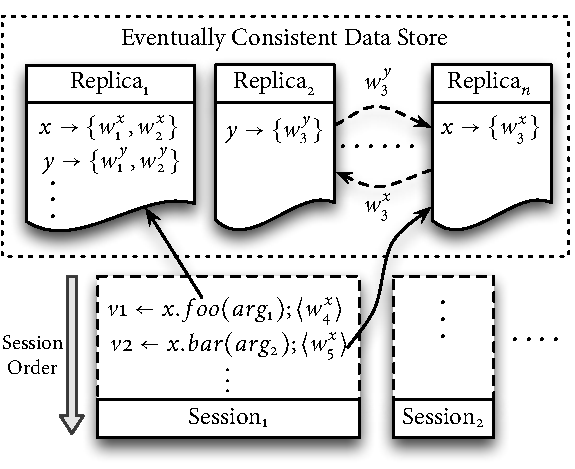
\includegraphics[width=0.7\columnwidth]{Figures/SystemModel}
\caption{\name system model.}
\label{fig:sysmod}
\end{figure}

In this section, we describe the system model and introduce the primitive
relations that our contract language is seeded with. Figure~\ref{fig:sysmod}
provides a schematic diagram of our system model. The distributed store is
composed of a collection of \emph{replicas}, each of which stores a set of
\emph{objects} ($x,y,\ldots$). We assume that every object is replicated at
every replica in the store. The state of an object at any replica is the set of
all updates (\emph{effects}) performed on the object. For example, the state of
$x$ at replica 1 is the ordered set composed of effects $w^x_1$ and $w^x_2$.

Each object is associated with a set of \emph{operations}. The clients interact
with the store by invoking operations on objects. The sequence of operations
invoked by a particular client on the store is called a \emph{session}. The
data store is typically accessed by a large number of clients (and hence
sessions) concurrently. Importantly, the clients are oblivious to which replica
an operation is applied to; the data store may choose to route the operation to
any replica in order to minimize latency, balance load, etc. For example, the
operations \emph{foo} and \emph{bar} invoked by the same session on the same
object, might end up being applied to different replicas because replica 1 (to
which \emph{foo} was applied) might be unreachable when the client invokes
\emph{bar}.

When \emph{foo} is invoked on a object $x$ with arguments \emph{arg}$_1$ at
replica 1, it simply \emph{reduces} over the current set of effects at that
replica on that object ($w^x_1$ and $w^x_2$), produces a result $v1$ that is
sent back to the client, and emits a \emph{single} new effect $w^x_4$ that is
appended to the state of $x$ at replica 1. Thus, every operation is evaluated
over a \emph{snapshot} of the state of the object on which it is invoked. In
this case, the effects $w^x_1$ and $w^x_2$ are \emph{visible} to $w^x_4$,
written logically as $\small \vis{w^x_1}{w^x_4} \wedge \vis{w^x_2}{w^x_4}$,
where $\small \visZ$ is the visibility relation between effects. Visibility is
an irreflexive and asymmetric relation, and only relates effects produced by
operations on the same object. Executing a read-only operation is similar
except that no new effects are produced. The effect added to a particular
replica is asynchronously sent to other replicas, and eventually merged into
all other replicas. Observe that this model does not assume a particular
resolution strategy for concurrent conflicting updates, and instead preserves
\emph{every} update. Update conflicts are resolved when an operation reduces
over the set of effects on an object at a particular replica.

Two effects $w^x_4$ and $w^x_5$ that arise from the same session are said to be
in \emph{session order} (written logically as $\small \so{w^x_4}{w^x_5}$).
Session order is an irreflexive, transitive relation. The effects $w^x_4$ and
$w^x_5$ arising from operations applied to the same object $x$ are said to be
under the \emph{same object} relation, written $\small \sameobj{w^x_4}{w^x_5}$.
Finally, we can associate every effect with the operation that generated the
effect with the help of a relation $\small \operZ$. In the current example,
$\small \oper{w^x_4}{foo}$ and $\small \oper{w^x_5}{bar}$ hold. For simplicity,
we assume all operation names across all object are distinct.

This model admits all the inconsistencies associated with eventual consistency.
The goal of this work is to identify the precise consistency level for each
operation such that application-level constraints are not violated. In the next
section, we will concretely describe the challenges associated with
constructing a consistent bank account on top of an \ecds. Subsequently, we
will illustrate how our contract and specification language, armed with the
primitive relations $\small \visZ$, $\small \soZ$, $\small \sameobjZ$ and
$\small \operZ$, mitigates these challenges.


\section{Motivation}
\label{sec:motivation}

Consider how we might implement a highly available bank account on top of an
\ecds, with the \emph{integrity} constraint that the balance must be
non-negative. We begin by implementing a bank account replicated data type
(RDT) in \name, and then describe the mechanisms to obtain the desired
correctness guarantees.

\subsection{RDT specification}

A key novelty in \name is that it allows the addition of new RDTs to the store,
which obviates the need for coercing the application logic to utilize the store
provided data types. In addition, \name treats the convergence semantics (i.e.,
\emph{how} conflicting updates are resolved) of the data type separately from
its consistency properties (i.e., \emph{when} updates become visible). This
separation of concerns permits \emph{operational} reasoning for conflict
resolution, and \emph{declarative} reasoning for consistency. The combination
of these techniques enhances the programmability of the store.

Let us assume that the bank account object provides three operations:
\cf{deposit}, \cf{withdraw} and \cf{getBalance}, with the assumption that the
withdraw fails if the account has insufficient balance. Every operation in
\name is of the following type, written in Haskell syntax:

\begin{codehaskell}
type Operation e a r = [e] -> a -> (r, Maybe e)
\end{codehaskell}

\noindent It takes a list of effects (the \emph{history} of updates to that
object), and an input argument, and returns a result along with an optional
effect (read-only operations return \cf{Nothing}). The new effect (if emitted)
is added to the state of the object at the current replica, and asynchronously
sent to other replicas. The implementation of the bank account operations in
\name is given in Figure~\ref{fig:ex}.

\begin{figure}
\vspace{-2.3mm}
\begin{codehaskell}
data Acc = Deposit Int | Withdraw Int | GetBal

getBalance :: [Acc] -> () -> (Int, Maybe Acc)
getBalance hist _ =
  let res = sum [x | Deposit x <- hist]
						- sum [x | Withdraw x <- hist]
	in (res, Nothing)

deposit :: [Acc] -> Int -> ((), Maybe Acc)
deposit hist amt = ((), Just dollar Deposit amt)

withdraw :: [Acc] -> Int -> (Bool, Maybe Acc)
withdraw hist v =
	if sel1 dollar getBalance hist () >= v
  then (True, Just dollar Withdraw v)
	else (False, Nothing)
\end{codehaskell}
\caption{Definition of a bank account expressed in Quelea.}
\label{fig:ex}
\end{figure}

The datatype \cf{Acc} represents the effect type for the bank account. The
function \cf{sum} returns the sum of elements in the list, and \cf{sel1}
returns the first element of a tuple. For each operation, \cf{hist} is a
\emph{snapshot} of the state of the object at some replica. In this sense,
every operation on the RDT is atomic, and thus permitting sequential reasoning
for implementing the RDTs. Here, \cf{getBalance} is a read-only operation,
\cf{deposit} always emits an effect, and \cf{withdraw} only emits an effect if
there is sufficient balance in the account. We have implemented a large corpus
of RDTs for realistic benchmarks including shopping carts, auction and
micro-blogging sites in few tens of lines of code.

\subsubsection{Summarization}
\label{sec:summarize}

Observe that the definition of \cf{getBalance} reduces over the \emph{entire
history} of updates to an account. If we are to realize an efficient
implementation of this bank account RDT, we need a \emph{summary} of the
account history. Intuitively, the current account balance summarizes the state
of an account. A bank account with the history \cf{[Deposit 10, Withdraw 5]} is
\emph{observably equivalent} to a bank account with a single deposit operation
\cf{[Deposit 5]}; we can replace the earlier history with the latter and a
client of the store would not able to tell the difference between the two.

This notion of observable equivalence can be generalized to other RDTs as well.
For example, a last-writer-wins register with multiple updates is equivalent to
a register with only the last write. Similarly, a set with a collection of add
and remove operations is equivalent to a set with a series of additions of live
elements from the original set. Since the notion of observable equivalence is
specific to each RDT, we expect the programmer to provide a summarization
function (\cf{summarize}) of type \cf{[e] -> [e]} for each RDT, as a part of
the RDT specification.

The summarization function for the bank account is \cf{summarize hist =
[Deposit \$ sel1 \$ getBalance hist ()]}. Given a bank account history
\cf{hist}, the \cf{summarize} function returns a new history with a single
deposit of the current account balance. We utilize the summarization function
to ensure that the state of an object remains summarized in each replica.

\subsection{Anomalies under Eventual Consistency}

Our goal is to choose the correct consistency level for each of the bank
account operations such that (1) the balance remains non-negative and (2) the
\cf{getBalance} operation never incorrectly returns a negative balance.

\begin{figure}[ht]
\vspace{-2mm}
\centering
\subfigure[Unsafe withdraw]{\label{fig:unsafeWithdrawAnomaly}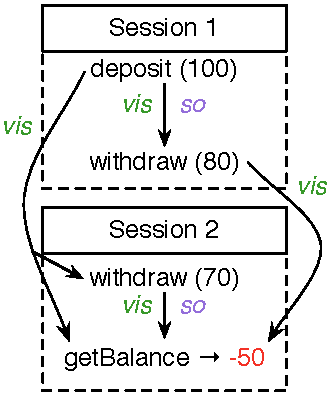
\includegraphics[width=0.34\columnwidth]{Figures/Motivation4}}
\hfill
\subfigure[Negative balance]{\label{fig:negativeBalanceAnomaly}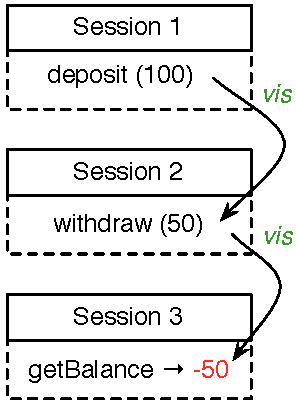
\includegraphics[width=0.31\columnwidth]{Figures/Motivation2}}
\hfill
\subfigure[Missing update]{\label{fig:missingUpdateAnomaly}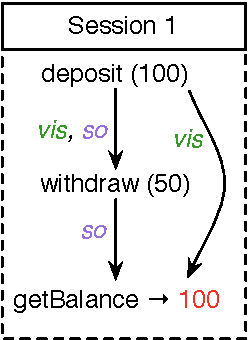
\includegraphics[width=0.26\columnwidth]{Figures/Motivation1}}
\caption{Anomalies possible under eventual consistency for the get balance operation.}
\label{fig:ba_anomalies}
\end{figure}

Consider the execution shown in Figure~\ref{fig:unsafeWithdrawAnomaly}. Assume
that all operations in the figure are on the same bank account object with the
initial balance being zero. Session 1 performs a \cf{deposit} of 100, followed
by a \cf{withdraw} of 80 in the same session. The \cf{withdraw} operation
witnesses\footnote{Although visibility and session
order relations relate effects, we have abused the notation in these examples
to relate operations, with the idea that the relations relate the effect
emitted by those operations} the deposit and succeeds. Subsequently, session 2 perform a \cf{withdraw}
operation, but importantly, due to eventual consistency, only witnesses the
\cf{deposit} from session 1, but not the subsequent withdraw. Hence, this
\cf{withdraw} also \emph{incorrectly} succeeds, violating the integrity
constraint. A subsequent \cf{getBalance} operation, that happens to witness all
the previous operations, would report a negative balance.

It is easy to see that preventing concurrent \cf{withdraw} operations
eliminates this anomaly. This can be done by insisting that \cf{withdraw} be
executed as a strongly consistent operation. Despite this strengthening,
the \cf{getBalance} operation may still incorrectly report a negative balance to
the user. Consider the execution shown in
fig.~\ref{fig:negativeBalanceAnomaly}, which consists of three concurrent
sessions performing a \cf{deposit}, a \cf{withdraw}, and a \cf{getBalance}
operation, respectively, on the same bank account object. As the {\sf vis} edge
indicates, operation \cf{withdraw(50)} in session 2 witnesses the effects of
\cf{deposit(100)} from session 1, concludes that there is sufficient balance,
and completes successfully. However, the \cf{getBalance} operation may only
witness this successful withdraw, but not the causally preceding \cf{deposit},
and reports the balance of negative 50 to the user.

Under eventual consistency, the users may also be exposed to other forms of
inconsistencies. Figure~\ref{fig:missingUpdateAnomaly} shows an execution where
the \cf{getBalance} operation in a session does not witness the effects of an
earlier \cf{withdraw} operation performed in the same session, possibly because
it was served by a replica that has not yet merged the \cf{withdraw} effect.
This anomaly leads the user to incorrectly conclude that the \cf{withdraw}
operation failed to go through.

Although it is easy to understand the reasons behind the occurrence of the
aforementioned anomalies, finding the appropriate fixes is not readily
apparent. Making \cf{getBalance} a strongly consistent operation is definitely
sufficient to avert anomalies, but is it really necessary? Given the cost of
enforcing strong consistency~\cite{DynamoDB, Pileus}, it is preferable to avoid
it unless there are no viable alternatives. Exploring the space of these
alternatives requires understanding the subtle differences in semantics of
various kinds of weak consistency alternatives.

\subsection{Contracts}

\name helps facilitate the mapping of operations to appropriate consistency
levels by letting the programmer declare application-level consistency
constraints as \emph{contracts}\footnote{\name exposes the contract
construction language as a Haskell library} (Figure~\ref{fig:contract-lang})
that axiomatically specify the set of allowed executions involving this
operation. In the case of the bank account, any execution that does not exhibit
the anomalies described in the previous section is a \emph{well-formed}
execution on the bank account object. By specifying the set of legal executions
for each data type in terms of a trace of operation invocations on that type,
\name\ ensures that all executions over that type are well-formed.

In our running example, it is clear that in order to preserve the integrity
constraint, the \cf{withdraw} operation must be strongly consistent.  That is,
given two \cf{withdraw} operations $a$ and $b$, either $a$ is visible to $b$ or
vice-versa. We express this application-level consistency requirement as a
contract ($\cv_w$) over \cf{withdraw}:

\vspace{-1em}
\begin{smathpar}
\begin{array}{l}
\forall (a : \rcf{withdraw}).~\sameobj{a}{\cureff} \Rightarrow a = \cureff \vee \vis{a}{\cureff} \vee \vis{\cureff}{a}
\end{array}
\end{smathpar}

\noindent Here, $\cureff$ stands for the effect emitted by the \cf{withdraw} operation.
The syntax $a:\rcf{withdraw}$ states that $a$ is an effect  emitted
by a \cf{withdraw} operation i.e., $\oper{a}{\rcf{withdraw}}$ holds.  The
contract specifies that if the current operation emits an effect $\cureff$,
then for any operation $a$ which was emitted by a \cf{withdraw} operation, it
is the case that $a = \cureff$ or $a$ is visible to $\cureff$, or vice versa.
Any execution on a bank account object that preserves the above contract for a
\cf{withdraw} operation is said to be derived from a correct implementation of
\cf{withdraw}.

\noindent For \cf{getBalance}, we construct the following contract ($\cv_{gb}$):

\vspace{-1em}
\begin{smathpar}
\begin{array}{l}
\forall (a:\rcf{deposit}), (b:\rcf{withdraw}), (c: \rcf{deposit} \vee \rcf{withdraw}). \\
\qquad (\vis{a}{b} \wedge \vis{b}{\cureff} \Rightarrow \vis{a}{\cureff}) \\
\qquad \wedge~ ((\soZ \cap \sameobjZ) (c,\cureff) \Rightarrow \vis{c}{\cureff})
\end{array}
\end{smathpar}

\noindent The expression $c:\rcf{deposit} \vee \rcf{withdraw}$ states that $c$
is an effect that was emitted either by a \cf{deposit} or a \cf{withdraw}
operation. If a \cf{withdraw} $b$ is visible to \cf{getBalance} $\cureff$, then
all \cf{deposit} operations $a$ visible to $b$ should also be visible to
$\cureff$. Intuitively, this prevents negative balance anomalies. Our contract
language provides operators to compose relations. The syntax $(R_1 \cap
R_2)(a,b)$ is equivalent to $R_1(a,b) \wedge R_2(a,b)$. The last line of the
above contract says that if a \cf{deposit} or a \cf{withdraw} operation
precedes a \cf{getBalance} operation in session order, and is applied on the
same object as the \cf{getBalance} operation, then it must be the case that the
\cf{getBalance} operation witnesses the effects of the preceding operations.

Finally, since there are no restrictions on when or how a \cf{deposit}
operation can execute, its contract is simply $\small \true$.

\subsection{From Contracts to Implementation}

Notice that the contracts for \cf{withdraw} and \cf{getBalance} only express
application-level consistency requirements, and make no reference to the
semantics of the underlying store. To write contracts, a programmer only needs
to reason about the semantics of the application under the \name system model.
The mapping of application-level consistency requirements to appropriate
store-level guarantees is done automatically behind-the-scene. How might one go
about ensuring that an execution adheres to a contract? The challenge is that a
contract provides a declarative (axiomatic) specification of an execution,
while what is required is an operational procedure for \emph{enforcing} its
implicit constraints.

One strategy would be to execute operations speculatively.  Here, operations
are tentatively applied as they are received from the client or other replicas.
We can maintain a runtime manifestation of executions, and check
well-formedness conditions at runtime, rolling back executions if they are
ill-formed. However, the overhead of state maintenance and the complexity of
user-defined contracts is likely to make this technique infeasible in practice.

We devise a static approach instead. Contracts are analyzed with the help of a
theorem prover, and statically mapped to a particular store-level consistency
property that the prover guarantees preserves contract semantics. We call this
procedure \emph{contract classification}. Given the variety and complexity of
store level consistency properties, the idea is that the system implementer
parameterizes the classification procedure by describing the store semantics in
the \emph{same} contract language as the one used to express the contract on
the operations. In the next section, we describe the contract language in
detail and describe the classification procedure for a particular store
semantics.


\section{Contract Language}
\label{sec:contract-lang}

% Contract Language Syntax
% ------------------------
\begin{figure}
\begin{smathpar}
\begin{array}{rclcl}
\multicolumn{5}{l}{
  {x,y,z} \in \mathtt{EffVar} \qquad
  {\cureff} \in \mathtt{CurEff} \qquad
  {\sf Op} \in \mathtt{OperName}
}\\
\cv 		& \in & \mathtt{Contract} 	& \coloneqq & \forall (x : \tau).\cv
        \ALT \pi \\
\tau		& \in	& \mathtt{EffType}	& \coloneqq &  {\sf Op}
        \ALT \tau \vee \tau \\
\pi			&	\in & \mathtt{Prop} & \coloneqq & \true \ALT R(x,y)
        \ALT \pi \vee \pi \\
			  & 		&	 &  \ALT & \pi \wedge \pi \ALT \pi \Rightarrow \pi \\
R				& \in & \mathtt{Relation}	& \coloneqq & \visZ \ALT \soZ
        \ALT \sameobjZ \ALT R^+ \\
				&			&	 &  \ALT & R \cup R \ALT R \cap R \\
\end{array}
\end{smathpar}
\caption{The Contract Language}
\label{fig:contract-lang}
\end{figure}


In this section, we formalize the contract language of \name, and describe our
contract classification scheme, which analyzes a contract and maps it to the
weakest store consistency level sufficient to satisfy its consistency
requirements.

% classifies contracts on the basis of the weakest
% store-level consistency guarantee

\subsection{Syntax}

The syntax of our core contract language is shown in Fig.
~\ref{fig:contract-lang}. The language is based on first-order logic (FOL), and
admits prenex universal quantification over typed effect variables. We use a
special effect variable ($\cureff$) to denote the effect of \emph{current
operation} - the operation for which a contract is being written. The type of
an effect is simply the name of the operation (eg: \cf{withdraw}) that induced
the effect. We admit disjuntion in types to let an effect variable range over
multiple operation names. The contract $\small \forall (a : \tau_1 \vee
\tau_2).~\psi$ is just syntactic sugar for $\small \forall a. (\oper{a}{\tau_1}
\vee \oper{a}{\tau_2}) \Rightarrow \psi$.

Quantifier-free propositions in our contract language are conjunctions,
disjunctions and implications of predicates expressing relations between pairs
of effect variables. The syntactic class of relations is seeded with primitive
$\visZ$, $\soZ$, and $\sameobjZ$ relations, and also admits derived relations
that are expressible as union, intersection, or transitive
closure\footnote{Strictly speaking, $R^{+}$ is not the transitive closure of
$R$, as transitive closure is not expressible in FOL.  Instead, $R^{+}$ in our
language denotes \emph{a} superset of transitive closure of $R$. Formally,
$R^{+}$ is any relation $R'$ such that forall $x$, $y$, and $z$, a) $R(x,y)
\Rightarrow R'(x,y)$, and b) $R'(x,y) \conj R'(y,z) \Rightarrow R'(x,z)$} of
primitive relations.  Commonly used derived relations are the \emph{same object
session order} ($\small \sooZ = \soZ ~\cap~ \sameobjZ$), and the \emph{same
object happens-before order} ($\small \hboZ = (\sooZ ~\cup~ \visZ)^+$).

\subsection{Semantics}

\begin{figure}
\begin{smathpar}
\stretcharraybig
\begin{array}{lclcl}
\multicolumn{5}{l}{
  {\eff} \in \mathtt{Effect} \qquad
  {\cv} \in \mathtt{Contract} \qquad
  \set{\eff} \in \mathtt{Effect\; Set}
}\\
\EffSoup & \in & \mathtt{EffSoup}	  & \coloneqq & \set{\eff} \\
\visZ, \soZ, &	\in & \mathtt{Relations} & \coloneqq &
  \set{\eff}\times\set{\eff} \\
\sameobjZ		&     &  & \\
{\E} 		& \in & \mathtt{ExecState}  & \coloneqq & \Exec \\
\end{array}
\end{smathpar}

\caption{An Axiomatic Execution}
\label{sem:contracts}
\end{figure}

In this section, we formally define what it means for an execution to
satisfy a contract.

\name contracts are constraints over axiomatic definitions of program
executions.Fig.~\ref{sem:contracts} summarizes artifacts relevant to
define an axiomatic execution. We formalize an axiomatic execution as
a tuple $\Exec$, where $\EffSoup$, called the \emph{effect soup}, is
the set of all effects generated during the program execution, and
$\visZ,\soZ,\sameobjZ \subseteq \EffSoup \times \EffSoup$ are
\emph{visibility}, \emph{session order}, and \emph{same object}
relations, respectively, witnessed over generated effects at run-time.

Note that the axiomatic definition an execution ($\E$) provides
interpretations for primitive relations (eg: $\visZ$) that occur free
in contract formulas, and also fixes the domain of quantification to
set of all effects ($\EffSoup$) observed during the program execution.
As such, $\E$ is a potential model for any first-order formula ($\cv$)
expressible in our contract language. If $\E$ is indeed a valid model
for $\cv$ (expressed using model-theoretic consequence relation as $\E
\models \cv$), we say that the execution $\E$ satisfied the contract
$\cv$:
\begin{definition}
An axiomatic execution $\E$ is said to satisfy a contract $\cv$ if and
only if $E \models \cv$.
\end{definition}

\subsection{Capturing Store Semantics}

An important aspect of our contract language is its ability to capture
store-level consistency guarantees, along with application-level
consistency requirements. Similar to~\cite{Burckhardt2014}, we can
rigorously define a wide variety of store semantics including those
that combine any subset of session and causality guarantees, and
multiple consistency levels.  However, for our purposes, we identify
three particular consistency levels -- eventual, causal, and strong,
commonly offered by many distributed stores with tunable consistency,
with increasing overhead in terms of latency and availability. For
each of the these three consistency levels, we capture the semantics
as a formula in our contract language, and informally describe the kind
of application-level consistency requirements that can met under the
consistency level:

% Indeed, the techniques presented here can be
% extended to other consistency stratifications. We assign each
% application-level contract into one of these following classes:

\begin{itemize}
\setlength{\itemsep}{2pt}

\item \textbf{Eventually consistency}: Eventually consistent operations can
  be satisfied as long as the client can reach at least one replica. For
  example, \cf{deposit} is an eventually consistent operation; its semantics
  does not require its action to manifest on all replicas before other
  operations in its session are allowed to proceed. While eventually
  consistent data store typically offer \emph{basic} eventual consistency
  with all possible anomalies, we assume that our store provides stronger
  semantics that remain highly-available~\cite{BailisHAT,COPS}; the store
  always exposes a causal cut of the updates. This semantics can be formally
  captured in terms of the following contract definition:

  \vspace{-1em}
  \begin{smathpar}
  \ecc = \forall a,b. ~\hbo{a}{b} \wedge \vis{b}{\cureff} \Rightarrow \vis{a}{\cureff}
  \end{smathpar}
  \noindent where $\small \hboZ = ((\soZ \cap \sameobjZ) \cup \visZ)^+$.

\item \textbf{Causal consistency}: Causally consistent operations
  are required to see a causally consistent snapshot of the object state,
  including the actions performed on the same session.  The latter
  requirement entails that if two operations $o_1$ and $o_2$ from the
  same session are applied to two different replicas $r_1$ and $r_2$,
  the second operation cannot be discharged until the effect of $o_1$ is
  merged with $o_2$ in both $r_1$ and $r_2$. The \cf{getBalance}
  operation requires causal consistency, as it requires the operations
  from the same session to be visible, which cannot be guaranteed under
  eventual consistency. We assume that causality is only tracked through
  operations on the same object; two operations in the same session but
  on different objects are considered causally unrelated under this
  definition. Stores typically avoid tracking causality across objects
  to mitigate overheads when causality tracking is unnecessary. The
  corresponding store semantics is captured by the contract $\ccc$
  defined below:

  \vspace{-1em}
  \begin{smathpar}
  \ccc = \forall a.~(\hboZ \cap \sameobjZ) (a,\cureff) \Rightarrow \vis{a}{\cureff}
  \end{smathpar}

\item \textbf{Strong Consistency}: Strongly consistent operations may block
  indefinitely under network partitions. An example is the total-order
  contract on \cf{withdraw} operation. The corresponding store semantics is
  captured by the $\scc$ contract definition:

  \vspace{-1em}
  \begin{smathpar}
  \scc = \forall a.~\sameobj{a}{\cureff} \Rightarrow \vis{a}{\cureff} ~\vee~ \vis{\cureff}{a} ~\vee~ a = \cureff
  \end{smathpar}

\end{itemize}

% SJ: not sure this is necessary, or appropriate here.
%% \noindent Observe that out contract language does not incorporate real (i.e.,
%% wall-clock) time. Hence, it cannot describe store
%% semantics such as recency or bounded-staleness
%% guarantees offered by certain stores~\cite{Pileus}.


% Contract classification rules
% ------------------------------
\newcommand{\DDe}[1]{#1}
\begin{figure}
\begin{smathpar}
\begin{array}{c}
\hspace{-0.5em}
\vspace{3mm}
\RuleTwo
{\DDe{\cv} \le \DDe{\scc}}
{{\sf WellFormed}(\cv)}  \qquad

\RuleTwo
{\DDe{\cv} \le \DDe{\ecc}}
{{\sf EventuallyConsistent}(\cv)} \\

\hspace{-0.5em}
\vspace{3mm}
\RuleTwo
{\DDe{\cv} \not\le \DDe{\ecc}
\quad \vdash \DDe{\cv} \le \DDe{\ccc}}
{{\sf CausallyConsistent}(\cv)} \qquad

\RuleTwo
{\DDe{\cv} \not\le \DDe{\ccc}
\quad \DDe{\cv} \le \DDe{\scc}}
{{\sf StronglyConsistent}(\cv)}

\end{array}
\end{smathpar}
\vspace{-5mm}

\caption{Contract classification.}
\label{sem:classify}
\end{figure}


\subsection{Contract Comparison and Classification}

Our goal is to map application-level consistency constraints on
operations to appropriate store-level consistency guarantees capable
of satisfying these constraints.  The ability to express both of them as
contracts in our contract language lets us compare and determine if
contract ($\cv_{op}$) of an operation ($op$) is weak enough to be
satisfied under a store consistency level identified by the contract
$\cv_{st}$. Towards this end, we define a binary \emph{weaker than}
relation for our contract language as following:

\begin{definition}
A contract $\cv_{op}$ is said to be weaker than $\cv_{st}$ (written $\cv_{op}
\le \cv_{st}$ ) if and only if $\Delta \vdash \cv_{st} \Rightarrow \cv_{op}$.
\begin{center}
\end{center}
\end{definition}

\vspace{-1em}
\noindent The $\Delta$ referred in the above defintion is a
conjunction of assumptions about the nature of primitive relations,
such as $\Rvis$ and $\Rso$ are irreflexive, and the happens-before
relation $\hbZ$ is acyclic. A \emph{well-formed} axiomatic execution
($\E$) is expected to satisfy these assumptions (i.e., $\E \models
\Delta$).

If the contract ($\cv_{op}$) of an operation ($op$) is \emph{weaker
than} a store contract ($\cv_{st}$), then constraints expressed by the
former are implied by guarantees provided by the later. Due to the
completeness of first-order logic\cite{completeness}, this means that
any well-formed execution ($\E$) that satisfies $\cv_{st}$ (i.e.,
$\E\models \cv_{st}$) also satisfies $\cv_{op}$ (i.e., $\E \models
\cv_{op}$). Consequently, it is safe to execute operation $op$ under
store consistency level captured by $\cv_{st}$.

Observe that the contracts $\scc$, $\ccc$ and $\ecc$ are themselves
totally ordered with respect to the $\le$ relation: $\ecc \le \ccc \le
\scc$.  This concurs with the intuition that any contract satisfiable
under $\ecc$ or $\ccc$ is satisfiable under $\scc$, and any contract
that is satisfiable under $\ecc$ is satisfiable under $\ccc$. However,
we are interested in the \emph{weakest} guarantee (among $\ecc$,
$\ccc$, and $\scc$) required to satisfy the contract. We define the
corresponding consistency level as the \emph{consistency class of the
contract}. The classification scheme is presented formally in
Figure~\ref{sem:classify}.

Along with three straightforward rules that classify contracts into
consistency classes, the classification scheme also presents a rule
that judges well-formedness of a contract. A contract is well-formed
if and only if it is satisfiable under $\scc$ - the strongest possible
consistency guarantee any store can provide. Otherwise, it is
considered ill-formed, and rejected statically.

\subsection{Soundness of Contract Classification}

In this section, we present a meta-theoretic result that certifies the
soundness of classification-based contract enforcement. To help us
state the result, we present an axiomatic model of the our system
described informally in Sec.~\ref{sec:sysmod}:

\begin{smathpar}
\begin{array}{lclcl}
\multicolumn{5}{l}{
  {op} \in \mathtt{Operation} \qquad
  \tau \in \mathtt{Consistency\; Class}
}\\
\cv(\tau) & \in & \mathtt{Store\; Contract\; of \; \tau} & \coloneqq & \scc,
  \ccc, \ecc\\
{\sigma} & \in & \mathtt{Session} & \coloneqq & \cdot \ALT (op,\tau); \sigma \\
\Sigma 	& \in & \mathtt{Session\;Soup}   & \coloneqq &
  \langle s,{\sigma} \rangle \pll \Sigma \ALT \emptyset \\
				&			&	\mathtt{Store}		  & \coloneqq & \E;\Sigma \\
\end{array}
\end{smathpar}

We model the system as a tuple $\E;\Sigma$, where the execution $\E$
captures the data store's current state of the execution, and
$\Sigma$, the session soup, is the set of concurrent client sessions
interacting with the store. A session is modeled simply as a sequence
of replicated data type operations ($op$), tagged with the consistency
class ($\tau$) of their contracts (as determined by the contract
classification scheme). We assume rewrite relation of form:

\vspace{-1.7em}
\begin{smathpar}
  \auxred{} {\E;\langle (op,\tau);\sigma \rangle \pll \Sigma} {\eff}
    {\E';\langle \sigma \rangle \pll \Sigma'}
\end{smathpar}

\noindent on the system state. The relation captures store's progress
in execution (from $\E$ to $\E'$) due to the application of an
operation ($op$) from one of the sessions in $\Sigma$ to a replica,
generating a new effect ($\eff$). If the resultant execution ($\E'$)
satisfies the store contract ($\cv(\tau)$) of $\tau$ (i.e., $\E
\models \cv(\tau)$), the we say that the store has \emph{enforced} the
contract $\cv(\tau)$ in the execution $\E'$.

With help of the axiomatic model, we now state the soundness of
contract enforcement as following:

\begin{theorem}[Soundness of Contract Enforcement]
\label{lem:core-preservation}
Let $\cv$ be a well-formed contract of a replicated data type operation $op$,
and let $\tau$ denote the consistency class of $\cv$ as determined by
the contract classification scheme. Forall well-formed execution
states $\E$, $\E'$ such that
$\auxred{} {\E;\langle (op,\tau);\,\sigma \rangle \pll \Sigma} {\eff}
 {\E';\langle \sigma \rangle \pll \Sigma}$
if $\E' \models [\eff/\cureff]\,\cv(\tau)$, then $\E' \models [\eff/\cureff]\,\cv$
\end{theorem}

The theorem states that if a data store correctly enforces $\scc$,
$\ccc$, and $\ecc$ contracts in all well-formed executions, then the
same store, extended with classification scheme, can enforce all
well-formed \name contracts. The proof of the theorem has been
relegated to our tech report~\cite{techrep} owing to space
constraints \footnote{Tech report also contains operational semantics of our
implementation of the data store, which concretizes the rewrite
relation ($\xrightarrow{}$), along with the proof that it correctly
enforces all \name contracts.}.




\section{Transaction Contracts}
\label{sec:txns}

While contracts on individual operations offer the programmer object-level
declarative reasoning, real-world scenarios often involve operations that span
multiple objects. In order to address this problem, several recent
systems~\cite{Walter,Burckhardt2012,BailisHAT} have proposed a variety of
transactions, with varying semantics, in order to compose operations on
multiple objects. However, given that classical transaction models such as
serializability and snapshot isolation require inter-replica coordination,
these systems espouse \emph{coordination-free transactions} that remain
available under network partitions, but only provide weaker isolation
guarantees. Coordination-free transactions have intricate consistency semantics
and widely varying runtime overheads. As with operation-level consistency, the
onus is on the programmer to pick the correct transaction kind; this selection
is complicated by operation consistency requirements.

\subsection{Syntax and Semantics Extension}
\label{sec:syn_sem_ext}

\name automates the choice of assigning the correct and most efficient
transaction isolation level. Similar to contracts on individual operations, the
programmer associates contracts with transactions, declaratively expressing its
consistency specification. We extend the contract language with a new term
under quantifier-free propositions - ${\small \txnZ}~S_1~S_2$, where $S_1$ and
$S_2$ are sets of effects, and introduce a new primitive equivalence relation
$\small \sametxnZ$ that holds for effects from the same transaction. $\small
\txn{a,b}{c,d}$ is just syntactic sugar for $\small \sametxn{a}{b} ~\wedge~
\sametxn{c}{d} ~\wedge~ \neg\sametxn{a}{c}$, where $a$ and $b$ considered to
belong to the \emph{current} transaction.

We assume that operations not part of any transaction belong to their own
unique transaction. While transactions may have varying isolation
guarantees, we make the standard assumption that all transactions provide
atomicity. Hence, we include the following axiom in $\Delta$: \[\small \forall
a,b,c.~\txn{a}{b,c} ~\wedge~ \sameobj{b}{c} ~\wedge~ \vis{b}{a} \Rightarrow
\vis{c}{a}\] \noindent The semantics of this contract is illustrated in
Figure~\ref{fig:txn_atomicity}.

\subsection{Transactional Bank Account}

In order to illustrate the utility of declarative reasoning for transactions,
consider an extension of our running example to use two accounts (objects) --
current ($c$) and savings ($s$). Each account provides operations
\cf{withdraw}, \cf{deposit} and \cf{getBalance}, with the same contracts as
defined previously. We consider two transactions -- \cf{save(amt)}, which
transfers \cf{amt} from current to savings, and \cf{totalBalance}, which
returns the sum of the balances of individual accounts. The \name code for the
transactions is given below:
\vspace{-1em}

\noindent \begin{minipage}[t]{0.53\columnwidth}
\begin{codehaskell}
save amt =
  x <- dollar(classify $\psi_1$)
  atomically x dollar do
    b <- withdraw c amt
    when b dollar deposit s amt
\end{codehaskell}
\end{minipage}
\begin{minipage}[t]{0.47\columnwidth}
\begin{codehaskell}
totalBalance =
  x <- dollar(classify $\psi_2$)
  atomically x dollar do
    b1 <- getBalance s
    b2 <- getBalance s
    return b1 + b2
\end{codehaskell}
\end{minipage}

\noindent $\cv_1$ and $\cv_2$ are the contracts on the corresponding
transactions. The function \cf{classify} assigns the contracts
\emph{statically} to one of the transaction isolation levels offered by the
store; \cf{\$()} is meta-programming syntax for splicing the result into the
program. The \cf{atomically} construct invokes the enclosing operations at the
given isolation level $x$, ensuring that the effects of the operations are made
visible atomically. Our goal is to ensure that \cf{totalBalance} returns the
result obtained from a consistent snapshot of the object states.

While making both transactions serializable would ensure correctness,
distributed stores rarely offer serializable transactions. Moreover,
serializability is unavailable and hinders scalability. As we will see, these
transactions can be satisfied with much weaker isolation guarantees. Despite
the atomicity offered by the transaction, anomalies are still possible. For
example, the two \cf{getBalance} operations in \cf{totalBalance} transactions
might be served by different replicas with distinct set of committed \cf{save}
transactions. If the first(second) \cf{getBalance} operation witness a
\cf{save} transaction that is not witnessed by the second(first)
\cf{getBalance} operation, then the balance returned will be less(greater) than
the actual balance. It is not immediately apparent which weakest isolation
guarantee will be sufficient to prevent the anomaly.

Instead, \name requires the programmer to simply state the consistency
requirement as a contract. Since we would like both the \cf{getBalance}
operations to witness the same set of \cf{save} transactions, we define the
constraint on \cf{totalBalance} transaction $\psi_2$ as:

\vspace{-1em}
\begin{smathpar}
\begin{array}{l}
\cv_{2} = \forall a:\rcf{getBalance}, b:\rcf{getBalance}, \\
\qquad (c:\rcf{withdraw} \vee \rcf{deposit}), (c:\rcf{withdraw} \vee \rcf{deposit}). \\
\qquad \txn{a,b}{c,d} ~\wedge~ \vis{c}{a} ~\wedge~ \sameobj{d}{b} \Rightarrow \vis{d}{b}
\end{array}
\end{smathpar}

\noindent The key idea in the above definition is that the $\txnZ$ primitive
allows us to relate operations on different objects.

The \cf{save} transaction only needs to ensure that the two writes it performs
are made visible atomically. Since this is ensured by combining them in a
transaction, \cf{save} does not require any additional constraints, and
$\psi_1$ is simply $\small \true$.

\subsection{Coordination-free Transactions}

\begin{figure}
\centering
\subfigure[Atomicity]{\label{fig:txn_atomicity}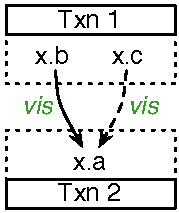
\includegraphics[width=0.25\columnwidth]{Figures/TxnAtomic}}
\hfill
\subfigure[Monotonic Atomic View]{\label{fig:txn_mav}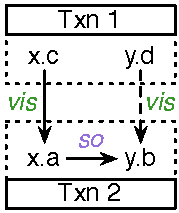
\includegraphics[width=0.25\columnwidth]{Figures/TxnMAV}}
\hfill
\subfigure[Repeatable Read]{\label{fig:txn_rr}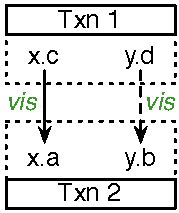
\includegraphics[width=0.25\columnwidth]{Figures/TxnRR}}
\caption{Semantics of transaction contracts. $x$ and $y$ are distinct objects.
The dotted line represents the visibility requested by the contracts.}
\label{fig:transaction}
\end{figure}

In order to illustrate the utility of transaction contract classification, we
identify three well-understood coordination-free transaction semantics -- Read
Committed (RC)~\cite{Berenson95}, Monotonic Atomic View (MAV)~\cite{BailisHAT}
and Repeatable Read (RR)~\cite{Berenson95}, and illustrate the classification
strategy. Our technique can indeed be applied to a different isolation level
lattice.

A transaction with ANSI RC semantics only witnesses committed operations. Let
us assume that the store buffers updates until all the updates from the
transaction are available at a replica. If the transaction commits, the
buffered updates are made visible. Otherwise, the buffered updates are
discarded. In particular, a store implementing RC does not require
inter-replica coordination. RC does not entail any further isolation
guarantees. We can express RC as follows:

\vspace{-1em}
\begin{smathpar}
\rcc = \forall a,b,c.~\txn{a}{b,c} \wedge \sameobj{b}{c} \wedge \vis{b}{a} \Rightarrow \vis{c}{a}
\end{smathpar}

\noindent Notice that the above definition is the same as the atomicity
guarantee of transaction described in Section~\ref{sec:syn_sem_ext}. The
\cf{save} is an example for RC transaction.

MAV semantics ensures that if some operation in a transaction $T_1$ witnesses
the effects of another transaction $T_2$, then subsequent operations in $T_1$
will also witness the effects of $T_2$. MAV semantics is useful for
maintaining the integrity of foreign key constraints, materialized views and
secondary updates. In order to implement MAV, a store only needs to keep track
of the set of transactions $S_t$ witnessed by the running transaction, and
before performing an operation at some replica, ensure that the replica
includes all the transactions in $S_t$. Hence, MAV is coordination-free. MAV
semantics is captured with the following contract:

\vspace{-1em}
\begin{smathpar}
\begin{array}{l}
\mavc = \forall a,b,c,d.~\txn{a,b}{c,d} ~\wedge~ \so{a}{b} ~\wedge~ \vis{c}{a} \\
\qquad\qquad\qquad\qquad ~\wedge~ \sameobj{d}{b} \Rightarrow \vis{d}{b}
\end{array}
\end{smathpar}

\noindent whose semantics is illustrated in the Figure~\ref{fig:txn_mav}.

RR semantics requires that the transaction witness a snapshot of the data store
state. Importantly, this snapshot can be obtained from any replica, and hence
RR is coordination-free. An example for such a transaction is the
\cf{totalBalance} transaction. The semantics of RR is captured by the following
contract:

\vspace{-1em}
\begin{smathpar}
\begin{array}{l}
\rrc = \forall a,b,c,d.~\txn{a,b}{c,d} ~\wedge~ \vis{c}{a} \\
\qquad\qquad\qquad\quad ~\wedge~ \sameobj{d}{b} \Rightarrow \vis{d}{b}
\end{array}
\end{smathpar}

\noindent whose semantics is illustrated in the Figure~\ref{fig:txn_rr}.

\subsection{Classification}

Similar to operation-level contracts, with respect to $\le$ relation, the
coordination-free transaction semantics described here form a total order:
$\rcc \le \mavc \le \rrc$. The transaction classification is also similar to
the operation-level contract classification presented in
Figure~\ref{sem:classify}; given a contract $\psi$ on a transaction, we start
from the weakest transaction contract $\rcc$, and progressively compare its
strength to the known transaction contracts until we find a isolation level
under which $\psi$ can be safely discharged. Otherwise, we report a type error.


\section{Implementation}
\label{sec:impl}

\name is implemented as a shallow extension of GHC Haskell and runs on top of
Cassandra, an off-the-shelf eventually consistent distributed data (or backing)
store responsible for all data management issues (i.e., replication, fault
tolerance, availability, and convergence).  Template Haskell is used to
implement static contract classification, and proof obligations are discharged
with the help of the Z3~\cite{Z3} SMT solver. Figure~\ref{fig:impl_mod}
illustrates the overall system architecture.

\begin{figure}
\begin{center}
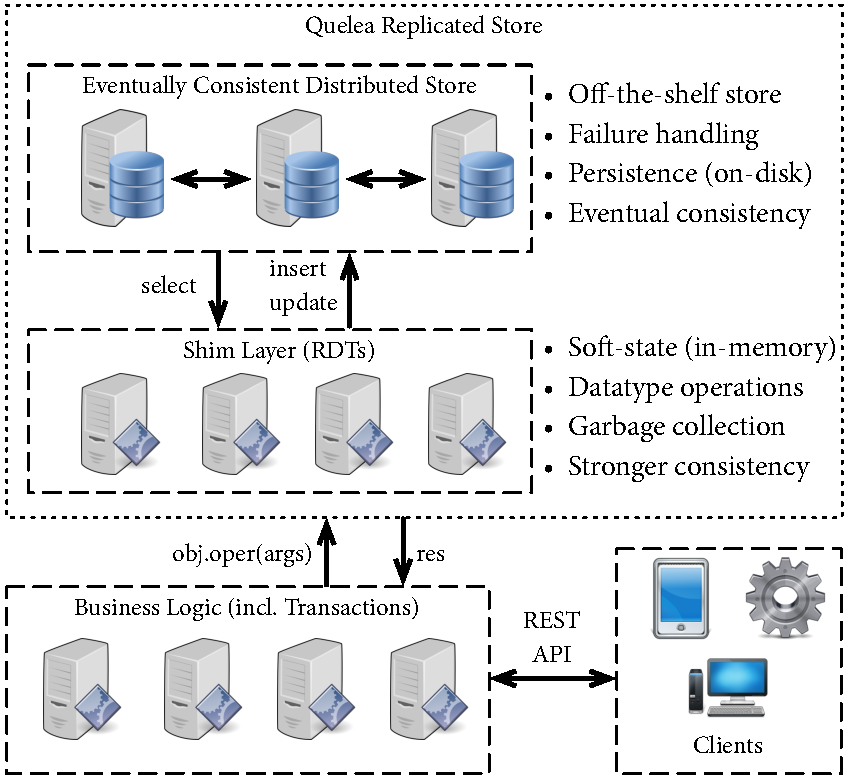
\includegraphics[width=\columnwidth]{Figures/ImplModel}
\end{center}
\caption{Implementation Model.}
\label{fig:impl_mod}
\end{figure}

Replicated data types and various consistency semantics are implemented and
enforced in the \emph{shim layer}. Our implementation supports eventual,
causal, and strong consistency for data type operations, and RC, MAV, and RR
semantics for transactions.  This functionality is implemented entirely on
top of the standard interface exposed by Cassandra. From an engineering
perspective, leveraging an off-the-shelf data store enables an
implementation comprising roughly only 2500 lines of Haskell code, which is
packaged as a library.

\subsection{Operation Consistency}

The shim layer maintains a causally consistent in-memory snapshot of a subset
of objects in the backing store, by explicitly tracking dependencies introduced
between effects due to visibility, session and same transaction relations.
Dependence tracking is similar to the techniques presented in~\cite{BoltOn}
and~\cite{Eiger}. Because Cassandra provides durability, convergence, and fault
tolerance, each shim layer node simply acts as a soft-state cache, with no
inter-node communication, and can safely be terminated at any point. Similarly,
new shim layer nodes can be spawned on demand.

Each effect generated as a result of an effectful operation on an object
inserts a new row $(o,\allowbreak e,\allowbreak txn,\allowbreak val,
\allowbreak deps)$ into the backing store, where $o$ and $e$ are object and
\emph{unique} effect identifiers, $txn$ is an optional transaction identifier,
and $val$ is the value associated with the effect (eg: \cf{Withdraw 50}).
$deps$ is the set of identifiers of \emph{dependencies} of this operation and
is defined as $deps(e) = \{e_1 \ALT \vis{e_1}{e} \wedge \neg(\exists
e_2.\vis{e_1}{e_2} \wedge \vis{e_2}{e})\}$. At any shim layer node, an effect
is included only if all of its dependencies are also included in that node.
This ensures that the state maintained by the shim layer node is causally
consistent. Our dependence tracking strategy ensures that \name does not track
every effect as the number of writes in the system grows.

The shim layer nodes periodically fetch updates from the backing store for
eventually consistent operations, and on-demand for causally consistent and
strongly consistent operations. Strongly consistent operations are performed
after obtaining exclusive leases on objects. The lease mechanism is implemented
with the help of Cassandra's support for conditional updates and expiring
columns.

\subsection{Transactions}

Cassandra does not provide general-purpose transactions. Since the transaction
guarantees provided by \name are coordination-free~\cite{BailisHAT}, we realize
efficient implementations by explicitly tracking dependencies between
operations and transactions. Importantly, the weaker isolation semantics of
transactions in \name permit transactions to be discharged if at least one shim
layer node is reachable.

\begin{figure}
\begin{center}
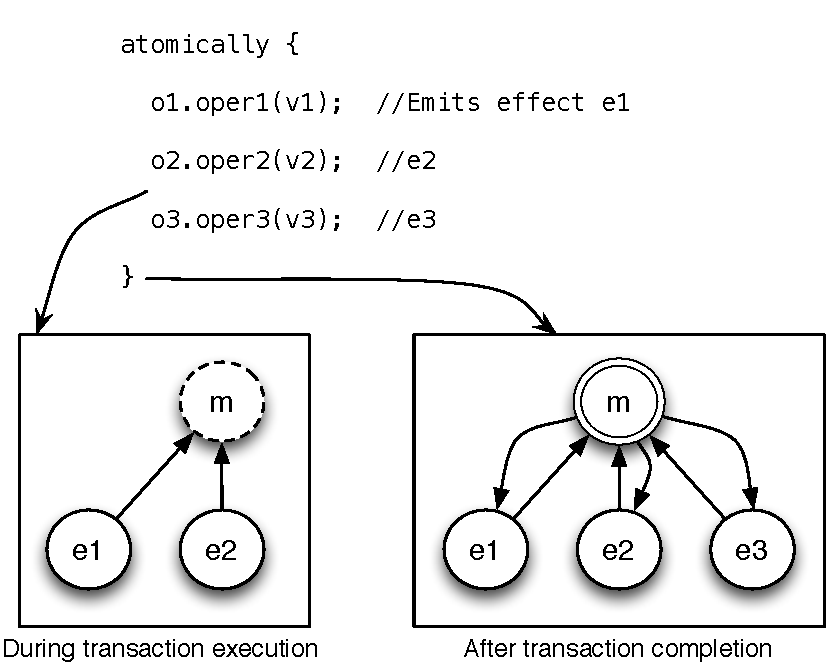
\includegraphics[width=0.7\columnwidth]{Figures/AtomicityImpl}
\end{center}
\caption{Implementing atomicity semantics. Dotted circle represents effects not
yet inserted into the backing store.}
\label{fig:atomicity_impl}
\end{figure}

\name implements atomic visibility by exploiting shim layer causality guarantee
-- an effect is included only if all the effects if depends on are also
included. Consider the example given in Figure~\ref{fig:atomicity_impl}. For
every transaction in \name, we instantiate a special transaction marker
effect $m$. But importantly, do not insert into the backing store. $m$ is
included as a dependence to every effect generated in the transaction. In the
figure, the graph on the left shows the state of the store in the middle of a
transaction. Each circle represents an effect. The dotted circle indicates that
the effect has been instantiated, but has not yet been inserted into the store.
Since the causally preceding effect $m$ has not yet been written to the store,
no operation will witness $e1$ and $e2$ while the transaction in progress.
After the transaction has finished execution, we insert $m$ into the backing
store, marking all the effects from the transactions as a dependence for $m$.
Now any replica which includes one of the effects from the transaction must
include $m$, and transitively must include every effect from the transaction.
This ensures atomicity and satisfies the RC requirement.

The above scheme prevents a transaction from witnessing its own effects. This
might conflict with the causality requirement on the operations. Hence,
transactions piggy-back the previous effects from the same transaction for each
request. MAV semantics is implemented by keeping track of the set of
transaction markers $M$ witnessed by the transaction, and before performing an
operation at some replica, ensuring that $M$ is a subset of the transaction
markers included at that replica. If not, the missing effects are synchronously
fetched. RR semantics is realized by capturing a optimized snapshot of the
state of some replica; each operation from an RR transaction is applied to this
snapshot state. Any generated effects are added to this snapshot.

\subsection{Summarization}

We utilize the \cf{summarize} function (\S~\ref{sec:summarize}) to summarize
the object state both in the shim layer node and the backing store, typically
when the number of effects on an object crosses a tunable threshold.
Shim layer summarization is straight-forward; a summarization thread takes the
local lock on the cached object, and replaces its state with the summarized
state. The shim layer node only remains unavailable for that particular object
during summarization (usually a few milliseconds).

Performing summarization in the backing store is more complicated since the
whole process needs to be atomic from a client's perspective, but Cassandra
does not provide multi-row transactions. Summarization in the backing store
involves deleting previously inserted rows and inserting new rows, where each
row corresponds to an effect. It is essential that concurrent client operations
are permitted, but are not allowed to witness the intermediate state of the
summarization process.

\begin{figure}
\begin{center}
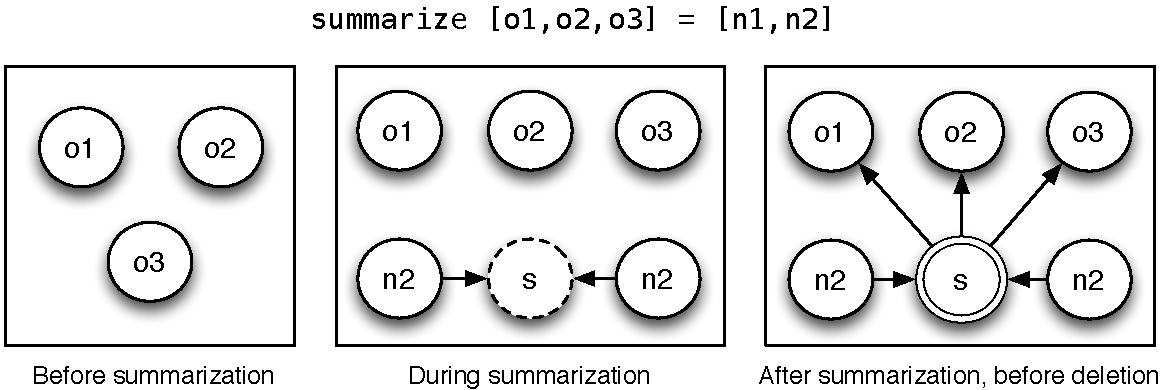
\includegraphics[width=\columnwidth]{Figures/SumDisk}
\end{center}
\caption{Summarization in the backing store. Dotted circle represents effects
not yet inserted into the backing store.}
\label{fig:impl_sum_disk}
\end{figure}

To this end, we adopt a novel summarization strategy that builds on the
causality property of the store. Figure~\ref{fig:impl_sum_disk} illustrates the
summarization strategy. Suppose the original set of effects on an object are
$o1$, $o2$ and $o3$. When summarized, the new effects yielded are $n1$ and
$n2$. We first instantiate a summarization marker $s$, and similar to
transaction marker, we do not insert it into the store immediately. We insert
the new effects $n1$ and $n2$, with strong consistency, including $s$ as a
dependence. Since $s$ is not yet in the store, the new effects are not made
visible to the clients. Then we insert $s$ with strong consistency, including
the original effects $o1$, $o2$ and $o3$ as dependence. Strongly consistent
insertions ensure that a shim layer node witnessing $s$ on some object must
also witness $n1$ and $n2$ on the same object. A shim layer node which
witnesses all the effects removes the original effects from its cache since
they are superseded by the new effects. Finally, the old effects are deleted
from the backing store. This process ensures that clients either witness the
old or the new effects, but not both; the summarization process appears to be
atomic from the clients perspective.


\section{Evaluation}

In this section, we evaluate \name programs and report their contract profile
as well as illustrating the performance benefits of fine-grained consistency
classification on operations and transactions. We also report on the impact of
the summarization. We implemented the following applications, which includes
RDTs as well as larger applications composed of severals RDTs:

\begin{itemize}

\item \textbf{LWW register}: A last-write-wins register that provides read and
write operations. Each write is associated with a timestamp, which is used to
resolve conflicting concurrent writes -- newer write wins.

\item \textbf{DynamoDB register}: A integer register that allows eventual and
strong puts and gets, conditional puts, increment and decrement operations.

\item \textbf{Bank account}: Our running example, with savings and current
accounts.

\item \textbf{Shopping list}: Collaborative shopping list which allows adding
and deleting items.

\item \textbf{Online store}: Models an online store with shopping cart and
dynamically changing item prices. Checkout process verifies that the custormer
only pays the accepted price.

\item \textbf{RuBis}: An ebay-like auction site~\cite{}. The application allows
users to browse items, bid for items on sale, and pay for items from a wallet
modelled after a bank account.

\item \textbf{Microblog}: A twitter-like microblogging site, modelled after
Twissandra~\cite{}. The application allows adding a new user, adding and
replying to tweets, following, unfollowing and blocking users, and fetching a
user's timeline, userline, followers and following.

\end{itemize}

\begin{table}
\setlength{\tabcolsep}{4pt}
{\sffamily \small
\begin{center}
\begin{tabular} {|l|r|r|r|r|r|r|r|r|}
\hline
{\bf Benchmark} & {\bf LOC} & {\bf \#T} & {\bf EC} & {\bf CC} & {\bf SC} & {\bf RC} & {\bf MAV} & {\bf RR} \\
\hline
{LWW Reg} & 108 & 1 & 2 & 2 & 2 & 0 & 0 & 0 \\
{DynamoDB} & 126 & 1 & 3 & 1 & 2 & 0 & 0 & 0 \\
{Bank Account} & 155 & 1 & 1 & 1 & 1 & 1 & 0 & 1 \\
{Shopping List} & 140 & 1 & 2 & 1 & 1 & 0 & 0 & 0 \\
{Online store} & 340 & 4 & 9 & 1 & 0 & 2 & 0 & 1 \\
{Rubis} & 640 & 6 & 14 & 2 & 1 & 4 & 2 & 0 \\
{Microblog} & 659 & 5 & 13 & 6 & 1 & 6 & 3 & 1 \\
\hline
\end{tabular}
\end{center} }
\caption{The distribution of classfied contracts. \#T refers to the number of
tables in the application. The columns 4-6 (7-9) represent operations
(transactions) assigned to this consistency (isolation) level.}
\label{tab:ctrts}
\end{table}

The distribution of contracts in these applications is given in
Table~\ref{tab:ctrts}. We see that majority of the operations and transactions
are classified as eventually consistent and RC, respectively. Operation
contracts are used to enforce integrity and visibility constraints on
individual fields in the tables. Transactions are mainly used to consistently
modify and access related fields across tables. The proof obligations
associated with contract classfication is discarged through the Z3 SMT Solver.
In \name, the contract classification process is completely performed compile
time and has no overheads at runtime. Across our benchmarks, classifying a
contract took 11.5 milliseconds on average.

\subsection{Performance}

In this section, we study the performance benefit of fine-grained contract
classification, and the impact of summarization optimization.

We deploy \name applications in \emph{clusters} where each cluster is composed
of 5 fully replicated Cassandra replicas within the same datacenter. We
instantiate one shim layer node for every cassandra replica, an place it on the
same VM as the cassandra replica. The clients are instantiated on the same data
center as the store, and run the transactions. We deploy the each node in the
cluster cluster on \cf{c3.4xlarge} Amazon EC2 instances with 16 virtual CPUs,
30GB memory, and 320GB of SSD storage. Our shim layer nodes are multi-threaded,
and we allocate 8 CPUs for each shim layer node. The clients also run on
\cf{c2.4xlarge} instances. We call this \cf{1DC} configuration. For our
geo-distributed experiments (\cf{2DC}), we instantiate 2 clusters, each with 5
nodes, and place the clusters on US-east (Virginia) and US-west (Oregon). The
average inter-region latency was 85ms.

\begin{figure*}
  \centering
  \subfigure[Bank account latency]{\label{grf:BA-lat}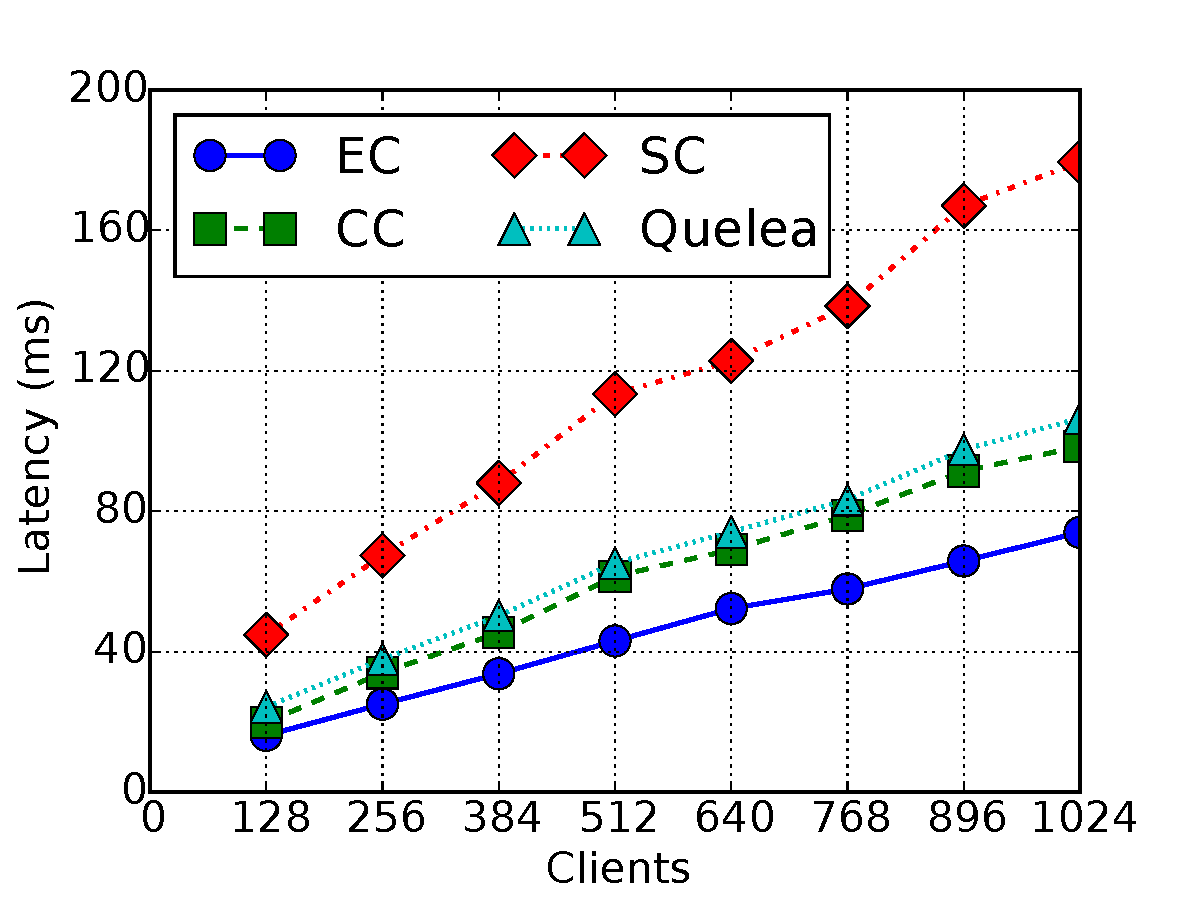
\includegraphics[width=0.252\textwidth]{graphs/BA-lat.pdf}}
  \subfigure[Bank account throughput]{\label{grf:BA-tp}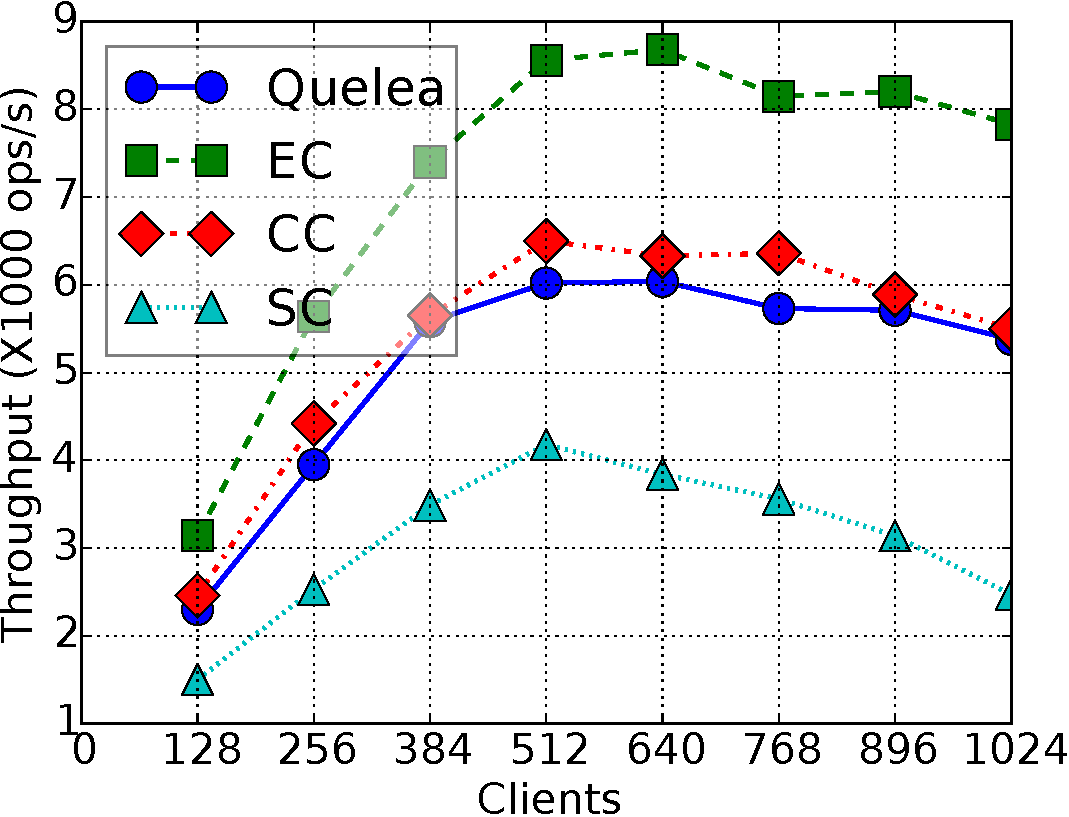
\includegraphics[width=0.24\textwidth]{graphs/BA-tp.pdf}}
  \subfigure[LWW transactions]{\label{grf:LWW-txn}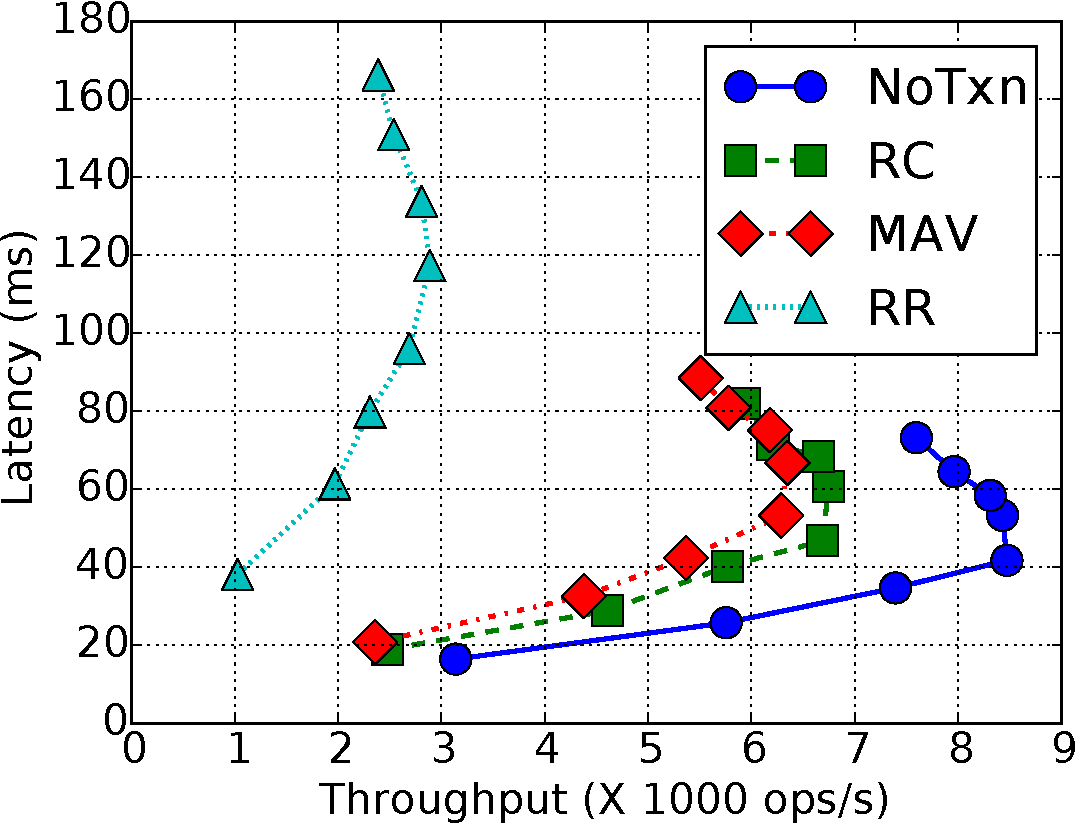
\includegraphics[width=0.24\textwidth]{graphs/LWW-txn.pdf}}
  \subfigure[Impact of summarization]{\label{grf:summarization}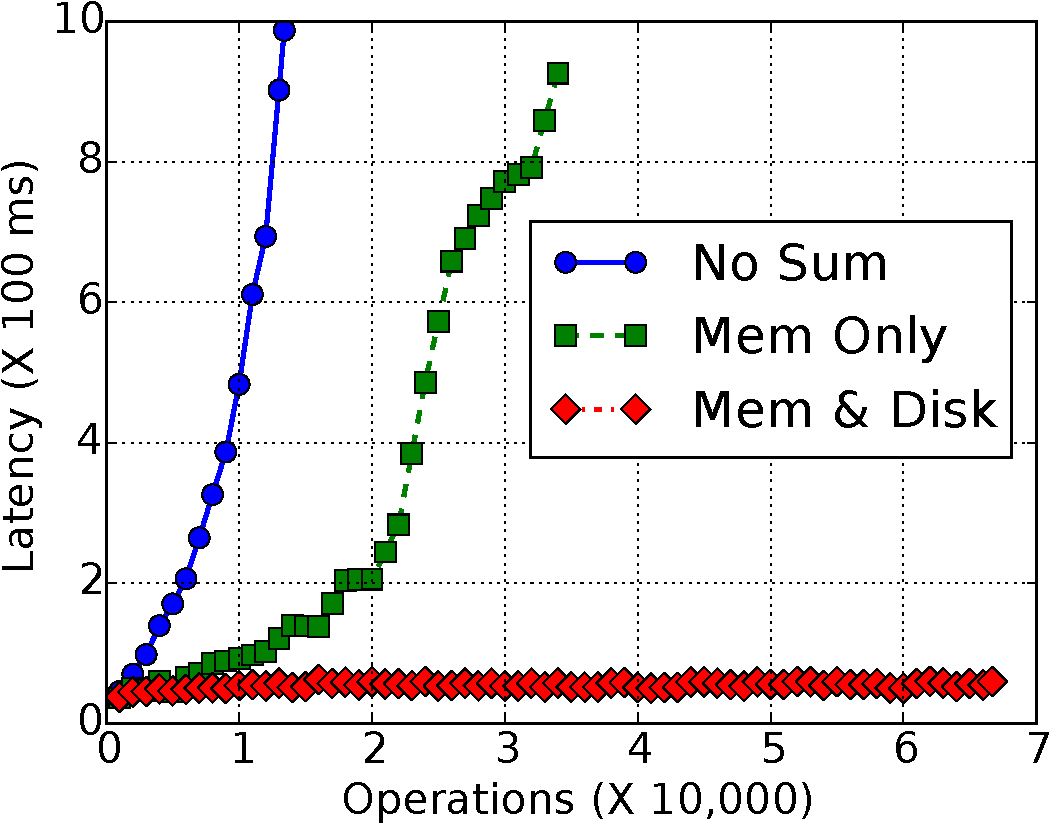
\includegraphics[width=0.235\textwidth]{graphs/summarization.pdf}}
	\caption{Quelea Performance.}
  \label{grf:LWW_perf}
\end{figure*}

Figure~\ref{grf:BA-lat} and~\ref{grf:BA-tp} analyzes the latency and throughput
of operations in bank account example as we increase the number of clients in
\cf{1DC} configuration. Our client workload was generated using YCSB
benchmark~\cite{}. The benchmark uniformly chose from 100,000 keys, where the
operation spread was 25\% withdraw, 25\% deposit and 50\% getBalance, which
corresponds to the default 50:50 read:write mix in YCSB. Here, the lines marked
EC and CC correspond to all operations being assigned EC and CC consistency
levels. These levels compromise correctness as withdraw has to be and SC
operation. The line SC corresponds to a configuration where all operations are
strongly consistent; this ensures application correctness. \name corresponds to
our implementation, which classifies operations based on their contracts.

Both \name and SC ensure correctness. However, with 512 clients, \name
implementation was within 41\% of latency and 18\% of throughput of EC, whereas
SC operations had 162\% higher latency and 52\% lower throughput than EC
operations. In \cf{2DC} configuration (not-shown), the average latency of SC
operations with 512 clients increased by 9.4$\times$ due to the cost of
geo-distributed coordination, whereas \name operations were only 2.2$\times$
slower, mainly due to the increased cost of \cf{withdraw} operations.
Importantly, the latency of \cf{getBalance} and \cf{deposit} remained almost
the same. This illustrates the benefit of fine-grained contract classification
in \name.

We compare the performance of different transaction isolation level choices in
Figure~\ref{grf:LWW-txn} using the LWW register. The numbers were obtained
under 1DC configuration. The YCSB workload was modified to issue 10 operations
per transaction, with the default 50:50 read:write mix. Each operation is
assumed to have eventual consistency. \cf{NoTxn} corresponds to a configuration
that does not use transactions. Compared to this RC is only 12\% shower in
terms of latency with 512 clients, where as RR is 2.3X slower. The difference
between RC and \cf{NoTxn} is due to the meta-data overhead of recording
transaction information in the object state. For RR transaction, the cost of
capturing and maintaining the snapshot in an RR transaction is the biggest
source of overhead.

We also compared the performance of EC LWW operations directly against
Cassandra (our backing store), which uses last-writer-wins as the only
convergence semantics. While Cassandra provides no stronger-than-eventual
consistency properties, \name was within 30\%(20\%) of latency(throughput) of
Cassandra with 512 clients, illustrating that the programmers only have to pay
a minimal overhead for the expressive and stronger \name programming model.

Finally, we study the impact of summarization in
Figure~\ref{grf:summarization}. We utilize 128 clients and a single \name
replica, with all the clients operating on the \emph{same} LWW register to
stress test the summarization mechanism. We utilize 50:50 read:write mix, and
33:33:33 EC:CC:SC mix. The shim layer cache (mem) of operations is summarized
every 64 updates, while the updates in the backing store (disk) are summarized
every 4096 updates. Each point in the graph represents the average latency of
the previous 1000 operations. Each experiment is run for 60s.

The results show that without summarization, the average latency of operations
increase exponentially to almost 1 second, and only 13K operations were
performed in a minute. Since every operation has to reduce over the set of all
previous operations, with a ever growing set, the operations take increasingly
more time to complete. With summarization only in memory, the performance still
degrades due to the cost of fetching all previous updates from the backing
store into the shim layer. Fetching the latest updates is essential for SC
operations. With both summarizations enabled, we see that the latency does not
increase over time, and we were able to perform 67K operations. This graph
illustrates the importance and effectiveness of summarization in \name.


\section{Related Work}
\label{sec:related}

Operation-based RDTs have been widely studied in terms of their algorithmic
properties~\cite{SSS,Burckhardt2014}, and several systems utilize this model to
construct distributed data structures~\cite{Cassandra,Bayou,Tango}. These
systems typically propose to implement the datatypes directly over a cluster of
nodes, and only focus on basic eventual consistency. Hence, these systems
implement custom solutions for durability and fault-tolerance. \name realizes
RDTs stronger consistency models on top of off-the-shelf eventually consistent
distributed stores. In this respect, \name is similar to~\cite{BoltOn} where
causal consistency is achieved through a shim layer on Cassandra, which
explicitly tracks and enforces depedencies between updates.
However,~\cite{BoltOn} does not support user-defined RDTs, automatic contract
classification and transactions.

Since eventual consistency alone is insufficient to build correct applications,
several systems~\cite{Bayou,Pileus,RedBlue} propose a lattice of stronger
consistency levels. Similarly, traditional database processing
systems~\cite{Berenson95} and their replicated variants~\cite{BailisHAT}
propose weaker isolation levels for performance. In these systems, the onus is
on the developer to choose the correct consistency(isolation) level for
operations(transactions). \name relieves the developer of this burden, and
instead expects contracts expressing declarative visibility requirements.

Our contract language is inspired by the axiomatic decription of RDT semantics
proposed by~\cite{Burckhardt2014}. While they use axioms for formal
verification of correctness of an RDT implementation, we utilize them as a
means for the user to express the desired consistency guarantees in the
application. Similar to their work, our contract language does not incorporate
real (i.e., wall-clock) time. Hence, it cannot describe store semantics such as
recency or bounded-staleness guarantees offered by certain
stores~\cite{Pileus}.

Program analysis has been proposed to relieve the annotation burden associated
with consistency classification.~\cite{Calm} identifies code regions that
require injection of coordination.~\cite{Sieve} automatically classifies
operations into strong and eventual consistency.~\cite{IConfluence} defines the
conditions under which an operation requires coordination. These works focus of
coarse-grained classification (eventual or strong), and do not focus on
transaction consistency. Indeed, we do see these approaches as a next step in
\name to automatically infer the contracts.


\section{Conclusions}
\label{sec:concl}

In this paper, we have presented \name a shallow Haskell extension for
declarative programming over eventually consistent data stores. The key idea of
\name is the automatic classification of fine-grained consistency contracts on
operations and distributed transactions with respect to the consistency and
isolation levels offered by the store. Our contract language is carefully
crafted from a decidable subset of first-order logic, enabling the use of
automatic theorem prover to discharge the proof obligations associated with
contract classification. We realize an instantiation of \name on top of
off-the-shelf distributed store, Cassandra, and illustrate the benefit of
fine-grained contract classification by implementing and evaluating several
scalable applications.


\bibliographystyle{abbrvnat}
\small
\bibliography{all}

\onecolumn
\appendix
\section{Appendix}
\label{sec:appendix}

\subsection{Soundness of Contract Classification}

We restate theorem ~\ref{thm:classification-sound} and provide its proof
below:

\begin{theorem}[Soundness of Contract Enforcement]
\label{lem:classification-sound}
Let $\cv$ be a well-formed contract of a replicated data type
operation $\mathit{op}$, and let $\tau$ denote the consistency class
of $\cv$ as determined by the contract classification scheme. For all
well-formed execution states $\E$, $\E'$ such that $\auxred{}
{\E,\langle op,\tau \rangle;\sigma \pll \Sigma} {\eff} {\E', \sigma
\pll \Sigma}$, if $\E' \models \cv_\tau[\eff/\cureff]$, then $\E'
\models \cv[\eff/\cureff]$
\end{theorem}
\begin{proof}
  Hypothesis:
  \begin{smathpar}
  \begin{array}{cr}
    \auxred{} {\E,\langle op,\tau \rangle;\sigma \pll \Sigma} {\eff}
    {\E', \sigma \pll \Sigma} & H\npp\\
    \E' \models \cv_\tau[\eff/\cureff] & H\npp\\
  \end{array}
  \end{smathpar}
  Since $\tau$ is the contract class of $\cv$, by inversion, we have
  $\cv \le \cv_\tau$. By the definition of $\le$ relation:
  \begin{smathpar}
  \begin{array}{cr}
    \Delta \vdash \forall \cureff.\,\cv_\tau \Rightarrow \cv & H\npp\\
  \end{array}
  \end{smathpar}
   Since $\eff$ denotes new effect, it is a fresh variable that does
   not occur free in $\Delta$. From $H2$, after instantiating bound
   $\cureff$ with $\eff$, we have:
  \begin{smathpar}
  \begin{array}{cr}
    \Delta \vdash \cv_\tau[\eff/\cureff] \Rightarrow \cv[\eff/\cureff]
      & H\npp\\
  \end{array}
  \end{smathpar}
  Due to the soundness of natural deduction for first-order logic,
  $H3$ implies that for all models $\mathcal{M}$ such that
  $\mathcal{M} \models \Delta$, if $\mathcal{M} \models
  \cv_\tau[\eff/\cureff]$ then $\mathcal{M} \models
  \cv[\eff/\cureff]$. Since $\E'$ is well-formed, we have:
  \begin{smathpar}
  \begin{array}{cr}
    \E' \models \Delta & H\npp\\
  \end{array}
  \end{smathpar}
  Proof follows from $H1$ and $H4$.
  \qed
\end{proof}

\subsection{Operational Semantics}
\renewcommand{\auxred}[4]{#1 \vdash #2 \;\xhookrightarrow{#3}\; #4 }

We now describe operational semantics of a data store that implements strong,
causal and eventual consistency guarantees. The semantics also serves as an
elegant representation of our implementation of \name.

Figure ~\ref{sem:oper} presents our semantics as concretization of the rewrite
relation ($\xrightarrow{}$) over execution state. Since we now have a concrete
store, we extend our system model with $\Theta$, a representation of the store
as a map from replicas to their local states. The local state of a replica $r$
(i.e., $\Theta(r)$) is a set of effects that are currently visible at $r$.  An
operation $op$ performed at replica $r$ can only witness the set of effects
($\Theta(r)$) visible at $r$. For the sake of clarity, we only consider a
single replicated object of well-defined type (for eg: a replicated object of
type \cf{BankAccount}) in our formalization.  Our semantics are parametric over
the specification of this replicated data type. Figure~\ref{sem:oper}
formalizes replicated data type (RDT) specification as tuple
$(\delta,\Ops,\Ctrts)$, where $\delta$ is the data type, $\Ops$ maps labels
($op$) of operations on $\delta$ to their definitions, while $\Ctrts$ maps them
to their consistency contracts ($\cv$). The definition of an operation is
expected to be a lambda expression, although we do not enforce this in our
formalization. For technical reasons, we tag each session with a session
identifier ($s$) and the sequence number ($i$) of the next operation in the
session.

The state of an operational execution ($\E$) is a tuple $\Exec$ where
$\EffSoup$ is a set of effects, and $\visZ,\soZ, \sameobjZ \subseteq \EffSoup
\times \EffSoup$ are \emph{visibility}, \emph{session order}, and \emph{same
object} relations over effects, respectively. We concretize an effect ($\eff$)
as a tuple $(s,i,op,v)$, which records the fact that $i^{th}$ action in session
with {\sf SessID} $s$, which is an operation $op$ on the replicated object, has
been successfully executed on some replica yielding a return value $v$. Note
that the combination of $s$ and $i$ uniquely identifies the effect. Session
order relation ($\soZ$) relates effects generated by the same session. An
effect $\eff = (s,i,op,v)$ is said to precede another effect $\eff' =
(s',i',op',v')$ in session order if and only if $s'=s$ and $i'\ge i$. Since we
only consider one replicated object in our formalization, the $\sameobjZ$
relation relates every pair of effects in the effect soup ($\EffSoup$). An
effect generated at a replica becomes visible at rest of the replicas
eventually.  If we denote the effect generated by the operation $op$ as
$\eff_{op}$, then $\Theta(r) \times \{\eff_{op}\} ~\subseteq~ \visZ$. Often, in
our formalization, we use $\visZ$ and $\soZ$ binary relations to obtain a set
of effects visible to a given effect $\eff$, or set of effects that precede a
given effect $\eff$ in the session order. As a syntactic convenience, whenever
$R$ is a binary relation, we write $R(\eff)$ to denote the set of all $\eff'$
such that $(\eff,\eff') \in R$.  Conversely, we write $R^{-1}(\eff)$ to denote
the set of all $\eff'$ such that $(\eff',\eff) \in R$.

Basic gurantee provided by the store is causal visibility, which is
captured by the rule $\rulelabel{EffVis}$ as a condition for an effect
to be visible at a replica. The rule makes an effect ($\eff$) visible
at a replica $r$ only after all the effects that causally precede
$\eff$ are made visible at $r$.  It is important to note that that
enforcing causal visibility does not require any inter-replica
coordination. Any eventually consistent store can provide causal
visibility while being eventually consistent.  Therefore, we do not lose
any generality by assuming that the store provides causal visiblity.

% Semantics
% ---------
\begin{figure}
\begin{smathpar}
\begin{array}{lclcl}
\multicolumn{5}{l}{
  {\eff} \in \mathtt{Effect} \qquad
  {op} \in \mathtt{Operation} \qquad
  {\cv} \in \mathtt{Contract}
}\\
\multicolumn{5}{l}{
  \set{\eff} \in \mathtt{Set\; of\; Effects} \qquad
  \tau \in \mathtt{Consistency\; Class}
}\\
%{op} & \in & {\sf Operation}& & \\
%\cv & \in & {\sf Contract} & &\\
\cv(\tau) & \in & \mathtt{Store\; Contract\; of \; \tau} & \coloneqq & \scc,
  \ccc, \ecc\\
%{a_s} & \in & \mathtt{Action} & \coloneqq &  \\
{\sigma} & \in & \mathtt{Session} & \coloneqq & \cdot \ALT (op,\tau); \sigma \\
%\eff & \in & \mathtt{Effect} & \coloneqq &  (s,~i,~op,~v)\\
\EffSoup & \in & \mathtt{EffSoup}	  & \coloneqq & \set{\eff} \\
\visZ, \soZ, &	\in & \mathtt{Relations} & \coloneqq &
  \set{\eff}\times\set{\eff} \\
%	\sameobjZ		&     &  & \\
{\E} 		& \in & \mathtt{ExecState}  & \coloneqq & (\EffSoup,\visZ,\soZ)\\
\Sigma 	& \in & \mathtt{Session\;Soup}   & \coloneqq &
  \langle s,{\sigma} \rangle \pll \Sigma \ALT \emptyset \\
				&			&	\mathtt{Store}		  & \coloneqq & \E;\Sigma \\
\end{array}
\end{smathpar}

\caption{Abstract model of a data store}
\label{sem:oper}
\end{figure}




Rule $\rulelabel{Oper}$ is an auxiliary reduction of the
\begin{smathpar}
\auxred{\Theta} {(\E,\langle s,i,op \rangle)} {r} {(\E',\eff)}
\end{smathpar}
\noindent Under the store configuration $\Theta$, the rule captures
the progress in execution (from $\E$ to $\E'$) due to the application
of operation $op$ to replica $r$ resulting in a new effect $\eff$.
The rule first constructs a \emph{context} for the application from
the local state ($\Theta(r)$) of the replica, by
projecting\footnote{{\textsf{ctxt*}} is auxiliary function
\textsf{ctxt} extended straightforwardly to set of effects} relevant
information from effects in $\Theta(r)$. It then substitutes the
definition ($\Ops(op)$) of the operation for its label ($op$), and
relies on the reduction relation ($\rdtredsto$) of the server-side
language to reduce the application $\Ops(op)(ctxt)$ to a value
$v'$.  Subsequently, the the attributes of execution state, namely
$\EffSoup$, $\visZ$, $\soZ$, and $\sameobjZ$ are extended to
incorporate the new effect ($\eff$).

If the operation $op$ is {\sf EventuallyConsistent}, we simply apply
the operation to any replica $r$. Since the store provides causal
visibility, eventually consistent operations are satisfiable under any
replica. If the operation is {\sf CausallyConsistent}, the operation
can be applied to a replica $r$ only if it already contains the
effects of all the previous operations from the same session. This
guarantee can be satisfied by applying all operations from the same
session to the same logical copy of the database.  If such a logical
copy is untenable, then the operation might block. Since the store is
assumed to converge eventually, the blocked causally consistent
operation guaranteed to unblock eventually.

A {\sf StronglyConsistent} operation expects sequential consistency.
That is, universe of all effects ($\EffSoup$) in an execution ($\E$)
must be partitionable into a set of effects that \emph{happened
before} $\eff$ and another set that \emph{happened after} $\eff$,
where $\eff$ is the effect generated by an strongly consistent
operation. The rule $\rulelabel{UA}$ enforces this sequencing in two
steps; firstly, it insists that the the strongly consistent operation
($op$) witness effects of all operations executed so far by requiring
the global set of effects $\EffSoup$ to be a subset of local state
($\Theta(r)$) of the replica ($r$) executing $op$. Secondly, the rule
requires the effect ($\eff$) generated by $op$ to be added to the
local state of every other replica in the store, so that further
operations on these replicas can witness the effect of $op$. Since
both these steps require global coordination among replicas, the store
is \emph{unavailable} during the time it is executing $op$.
% However, it must be noted that executing strongly consistent
% operation does not entail the convergence of local states of all
% replicas; it simply means that there is one replica ($r$) whose
% local state is the upper bound of local states of all replicas, and
% there exists a set containing atleast one effect ($\eff$), which is
% their lower bound.

\subsection{Soundness of Operational Semantics}

Our main meta-theoretic result guarantees the soundness of our operational
semantics in enforcing $\ecc$, $\ccc$, and $\scc$ consistency guarantess by
ensuring that every reduction step preserves correctness of operational
execution.

\begin{theorem}[Soundness preservation]
\label{lem:core-preservation}
Let $\E$ be a well-formed operational execution state, and $\tau$ denote a
contract class.  If:
\begin{smathpar}
\E; \Theta; \langle s,i,\langle op,\tau \rangle;
\sigma \rangle \pll \Sigma \xhookrightarrow{\eff} \E'; \Theta';
\langle s,i,\sigma \rangle \Sigma'
\end{smathpar}
then (\romannumeral 1) $\E'$ is well-formed, and (\romannumeral 2)
$\E' \models \cv_{\tau}[\eff/\cureff]$
\end{theorem}


\end{document}
